% ============================================
% Project Documentation Template
% Based on: Uniba - Collab Thesis Template
% Developed and maintained by Giulio Mallardi
% https://collab.uniba.it | © 2025 Collab
% Adapted for project documentation
% ============================================
\PassOptionsToPackage{table, dvipsnames}{xcolor}
\documentclass[a4paper,oneside,11pt]{report}
\usepackage[left=2.2cm,right=2.2cm,top=2.2cm,bottom=2.2cm]{geometry}
\usepackage[T1]{fontenc}
\usepackage[utf8]{inputenc}
\usepackage[english]{babel}
\usepackage{xspace}
\usepackage{graphicx}
\usepackage{tikz}
\usetikzlibrary{positioning, shapes.geometric}
\usepackage{pgfplots}
\pgfplotsset{compat=1.18}
\usepackage[font=small,skip=1pt]{caption}
\usepackage{subcaption}
\usepackage{hyperref}
\hypersetup{
    colorlinks = true,
    allcolors=black
}
%This equals 1.3 linespacing in Word (compacted)
\linespread{1.15}

% Reduce spacing around floats and between text/floats
\setlength{\textfloatsep}{8pt plus 2pt minus 2pt}
\setlength{\floatsep}{8pt plus 2pt minus 2pt}
\setlength{\intextsep}{8pt plus 2pt minus 2pt}
\setlength{\abovecaptionskip}{4pt}
\setlength{\belowcaptionskip}{2pt}

\usepackage{fancyhdr}
\usepackage{ifthen}

% --- GitHub icon in page header (top right, clickable) ---
\usepackage{fontawesome5}
\pagestyle{fancy}
\fancyhf{}
\fancyhead[R]{\href{https://github.com/icekern/DB}{\color{black!60}{\Large\faGithub}}}
\fancyfoot[C]{\thepage}
\renewcommand{\headrulewidth}{0pt}
\fancypagestyle{plain}{%
  \fancyhf{}%
  \fancyhead[R]{\href{https://github.com/icekern/DB}{\color{black!60}{\LARGE\faGithub}}}%
  \fancyfoot[C]{\thepage}%
  \renewcommand{\headrulewidth}{0pt}%
}

% --- Pacchetti aggiuntivi per documentazione di progetto ---
\usepackage{amsmath, amssymb, amsthm}
\usepackage{booktabs}
\usepackage{tabularx}
\usepackage{longtable}
\usepackage{ltablex}
\usepackage{multirow}
\usepackage{array}
\usepackage{enumitem}
\usepackage{xcolor}

% --- Code listings (alternativa a minted, non richiede Python/Pygments) ---
\usepackage{listings}
\lstdefinestyle{unibastyle}{
    basicstyle=\ttfamily\small,
    keywordstyle=\color{blue}\bfseries,
    commentstyle=\color{gray}\itshape,
    stringstyle=\color{red!70!black},
    numberstyle=\tiny\color{gray},
    breaklines=true,
    frame=single,
    rulecolor=\color{black!30},
    numbers=left,
    tabsize=4,
    showstringspaces=false,
    captionpos=b,
    backgroundcolor=\color{black!3}
}
\lstset{style=unibastyle}

% SQL language
\lstdefinelanguage{SQL}{
    morekeywords={SELECT, FROM, WHERE, INSERT, INTO, VALUES, UPDATE, SET, DELETE,
                  CREATE, TABLE, ALTER, DROP, INDEX, VIEW, JOIN, INNER, LEFT, RIGHT,
                  OUTER, ON, AND, OR, NOT, IN, BETWEEN, LIKE, IS, NULL, AS, ORDER,
                  BY, GROUP, HAVING, DISTINCT, UNION, ALL, EXISTS, CASE, WHEN, THEN,
                  ELSE, END, PRIMARY, KEY, FOREIGN, REFERENCES, CHECK, DEFAULT,
                  CONSTRAINT, UNIQUE, CASCADE, TRIGGER, PROCEDURE, FUNCTION, BEGIN,
                  COMMIT, ROLLBACK, TRANSACTION, GRANT, REVOKE, WITH, RECURSIVE,
                  INTEGER, VARCHAR, CHAR, TEXT, BOOLEAN, DATE, TIMESTAMP, FLOAT,
                  DECIMAL, NUMERIC, SERIAL, BIGINT, SMALLINT, REAL, COUNT, SUM,
                  AVG, MIN, MAX, LIMIT, OFFSET, ASC, DESC, IF, REPLACE, TEMPORARY,
                  SCHEMA, DATABASE, USE, SHOW, DESCRIBE, EXPLAIN},
    sensitive=false,
    morecomment=[l]{--},
    morecomment=[s]{/*}{*/},
    morestring=[b]',
    morestring=[b]"
}

% Python language (used in Chapter 5 for Flask code snippets)
\lstdefinelanguage{Python}{
    morekeywords={def, return, if, else, elif, for, while, import, from, as, class,
                  try, except, finally, with, raise, pass, None, True, False, not,
                  and, or, in, is, lambda, yield, global, nonlocal, assert, del,
                  break, continue, exec, print},
    sensitive=true,
    morecomment=[l]{\#},
    morecomment=[s]{"""}{"""},
    morestring=[b]',
    morestring=[b]"
}

% --- Custom Boxes (tcolorbox) ---
% Three visual styles only: GREY (code/reference), VIOLET (reasoning/assumption), BLUE (info)
\usepackage[most]{tcolorbox}

% ===== STYLE 1: GREY — Code and reference text =====

\newtcblisting{sqlbox}[1][]{
    enhanced,
    breakable,
    listing only,
    listing options={
        language=SQL,
        basicstyle=\ttfamily\small,
        keywordstyle=\color{blue!70!black}\bfseries,
        stringstyle=\color{red!60!black},
        commentstyle=\color{black!45}\itshape,
        breaklines=true,
        showstringspaces=false,
        tabsize=4
    },
    colback=black!3!white,
    colframe=black!35,
    fonttitle=\bfseries\ttfamily\small,
    title={SQL},
    attach boxed title to top left={yshift=-2mm, xshift=5mm},
    boxed title style={colback=black!45, colframe=black!45},
    sharp corners,
    boxrule=0.8pt,
    left=4mm, right=4mm, top=5mm,
    before skip=6pt, after skip=6pt,
    #1
}

% Specification box (green, for requirement quotes)
\newtcolorbox{tracebox}[1][]{
    enhanced,
    colback=green!4!white,
    colframe=green!50!black,
    fonttitle=\bfseries\small,
    title={Specifications},
    attach boxed title to top left={yshift=-2mm, xshift=5mm},
    boxed title style={colback=green!50!black, colframe=green!50!black},
    sharp corners,
    boxrule=0.8pt,
    left=4mm, right=4mm, top=5mm,
    before skip=6pt, after skip=6pt,
    borderline west={3pt}{-4pt}{green!50!black},
    #1
}

% Generic grey highlight (no title, italic)
\newtcolorbox{highlightbox}[1][]{
    enhanced,
    colback=black!3!white,
    colframe=black!35,
    boxrule=0pt,
    borderline west={4pt}{0pt}{black!40},
    sharp corners,
    left=6mm, right=4mm, top=2mm, bottom=2mm,
    before skip=6pt, after skip=6pt,
    fontupper=\itshape,
    #1
}

% ===== STYLE 2: VIOLET — Reasoning and assumptions =====

\newtcolorbox{reasoningbox}[1][]{
    enhanced,
    colback=violet!4!white,
    colframe=violet!55!black,
    fonttitle=\bfseries\small,
    title={Assumption / Design Reasoning},
    attach boxed title to top left={yshift=-2mm, xshift=5mm},
    boxed title style={colback=violet!55!black, colframe=violet!55!black},
    sharp corners,
    boxrule=0.8pt,
    left=6mm, right=4mm, top=5mm,
    before skip=6pt, after skip=6pt,
    borderline west={4pt}{0pt}{violet!55!black},
    #1
}

\newtcolorbox{assumptionbox}[1][]{
    enhanced,
    colback=violet!4!white,
    colframe=violet!55!black,
    fonttitle=\bfseries\small,
    title={Assumption / Design Reasoning},
    attach boxed title to top left={yshift=-2mm, xshift=5mm},
    boxed title style={colback=violet!55!black, colframe=violet!55!black},
    sharp corners,
    boxrule=0.8pt,
    left=6mm, right=4mm, top=5mm,
    before skip=6pt, after skip=6pt,
    borderline west={4pt}{0pt}{violet!55!black},
    #1
}

% ===== STYLE 3: BLUE — Informational notes =====

\newtcolorbox{infobox}[1][]{
    enhanced,
    colback=blue!4!white,
    colframe=blue!55!black,
    fonttitle=\bfseries\small,
    title={Info},
    attach boxed title to top left={yshift=-2mm, xshift=5mm},
    boxed title style={colback=blue!55!black, colframe=blue!55!black},
    sharp corners,
    boxrule=0.8pt,
    left=4mm, right=4mm, top=5mm,
    before skip=6pt, after skip=6pt,
    #1
}

% Legacy aliases — all map to one of the three styles above
\newtcolorbox{notebox}[1][]{
    enhanced,
    colback=blue!4!white,
    colframe=blue!55!black,
    fonttitle=\bfseries\small,
    title={Note},
    attach boxed title to top left={yshift=-2mm, xshift=5mm},
    boxed title style={colback=blue!55!black, colframe=blue!55!black},
    sharp corners,
    boxrule=0.8pt,
    left=4mm, right=4mm, top=5mm,
    before skip=6pt, after skip=6pt,
    #1
}

% ============================================
%  METADATA – EDIT THESE FIELDS
% ============================================
\def\dept{DEPARTMENT OF COMPUTER SCIENCE}
\def\course{MASTER'S DEGREE IN COMPUTER SCIENCE}

\def\projecttitle{ConferenceHub Inc.}                        % <-- Project title
\def\projectsubtitle{Project Documentation}         % <-- Subtitle
\def\authorname{Andrea Porcelli}                            % <-- Your name
\def\subject{DATABASE}                             % <-- Subject
\def\docente{Prof. Antonio Pellicani}                   % <-- Professor name
\def\annoacc{2025 - 2026}                          % <-- Academic year

% Title page labels
\def\beforeauthor{STUDENT:}
\def\beforetitle{COURSE DOCUMENTATION \\}
\def\beforeprof{PROFESSOR:}
\def\beforeannoacc{ACADEMIC YEAR}

% ============================================
%  CLEARDOUBLEPAGE FIX
% ============================================
\makeatletter
\def\cleardoublepage{\clearpage\if@twoside \ifodd\c@page\else
    \hbox{}
    \vspace*{\fill}
    \vspace{\fill}
    \thispagestyle{empty}
    \newpage
    \if@twocolumn\hbox{}\newpage\fi\fi\fi}
\makeatother


% ============================================
%  DOCUMENT
% ============================================
\begin{document}

% --- Title Page (stile Collab UNIBA) ---
\begin{titlepage}
	\begin{tikzpicture}[remember picture,overlay]
		\centering
		\node[yshift=-6 cm] (logo) at (current page.north) {\includegraphics[width=0.75\linewidth]{images/logos/uniba.pdf}};
			\node[text width=50em,yshift=0.25cm, align = center, below = of logo](dipartimento){\normalsize \dept};
			\node[text width=40em, align = center, yshift=.55cm,below = of dipartimento](coursename){\normalsize \course};
		\node[text width=35em,align = center,  yshift=1.2cm,below = of coursename](line){\par\noindent\rule{\textwidth}{0.4pt}};
		\node[text width=40em, align = center, yshift=.55cm,below = of line](lia){\normalsize \beforetitle \xspace \subject };
		
  \node[text width=40em, align = center, yshift=-0.5cm,below = of lia](title){\bfseries \parbox{12cm}{\fontsize{21pt}{20pt}\selectfont \centering \projecttitle\par}};
  
  \node[text width=40em, align = center, yshift=0.3cm,below = of title](subtitle){\large \textit{\projectsubtitle}};

	\node[text width=35em, align = left, yshift=-0.5cm,below = of subtitle](proftit){\normalsize \textbf{\beforeprof} };
 	\node[text width=35em, align = left, yshift=1cm,below = of proftit](prof){\large \docente};
      
		\node[text width=35em, align = right, yshift=-0.5cm,below = of subtitle](candidatetit){\normalsize \textbf{\beforeauthor}};
		 \node[text width=35em, align = right, yshift=1cm,below = of candidatetit](candidate){\large \authorname};

  \node[text width=35em,align = center,  yshift= -3cm,below = of candidate](line2){\par\noindent\rule{\textwidth}{0.4pt}};
	
  \node[text width=50em, align = center, yshift=0.5cm,below = of line2](year){\large \beforeannoacc\xspace \annoacc};
	\end{tikzpicture}
\end{titlepage}


\cleardoublepage

% --- Table of Contents ---
\pagenumbering{roman}
\tableofcontents
\cleardoublepage

% ============================================
%  CONTENT
% ============================================
\pagenumbering{arabic}
\setcounter{page}{1}

% --- Introduction (unnumbered) ---
\addcontentsline{toc}{chapter}{Introduction}
\chapter*{Introduction}

This document is the project report for the Database course at the Department of Computer Science, University of Bari Aldo Moro.

The project is about designing and building a database for a company called ConferenceHub Inc. that manages academic conferences. The document is divided into chapters: requirements analysis, conceptual design (ER), logical design, physical implementation in Oracle SQL, web application, and a bonus chapter on data warehousing.

\section*{Box Types Used in This Document}

In this document we use colored boxes to separate different types of content. Each color has a specific meaning:

\begin{itemize}[itemsep=6pt]
    \item \textbf{\textcolor{green!50!black}{Green} --- Specifications.} Text taken directly from the original requirements.

    \item \textbf{\textcolor{violet!55!black}{Violet} --- Assumption / Design Reasoning.} Explains a design choice or an assumption we made.

    \item \textbf{\textcolor{blue!55!black}{Blue} --- Info.} Extra context or useful notes.

    \item \textbf{\textcolor{black!45}{Grey} --- SQL Code.} SQL code with syntax highlighting.
\end{itemize}

Here is an example of each box:

\begin{tracebox}
This is a green Specifications box. It shows text taken from the requirements.
\end{tracebox}

\begin{reasoningbox}
This is a violet Assumption / Design Reasoning box. It explains a design decision or an assumption.
\end{reasoningbox}

\begin{infobox}
This is a blue Info box. It gives additional context or clarifications.
\end{infobox}

\begin{highlightbox}
This is a grey highlight box, used for short formulas or patterns worth remembering.
\end{highlightbox}


% --- Chapters ---
\chapter{Requirements Analysis}
\label{ch:requirements_analysis}

In this chapter we analyze the original specification using the standard 8-phase method. Each step cleans up and organizes the text so we can use it in the next phase.

The eight phases are:
\begin{enumerate}[itemsep=4pt, topsep=6pt]
    \item \textbf{Choose the right level of abstraction}
    \item \textbf{Standardize sentence structure}
    \item \textbf{Linearize and split articulated phrases}
    \item \textbf{Identify homonyms and synonyms}
    \item \textbf{Make explicit references between terms}
    \item \textbf{Build a glossary}
    \item \textbf{Reorganize phrases by keyword}
    \item \textbf{Separate data specifications from functional requirements}
\end{enumerate}

\section{Requirements Gathering Output}
\label{sec:requirements_gathering_output}

Below is the original specification text:

\begin{tracebox}
Each conference organized by the company ``ConferenceHub Inc.'' is identified by an acronym and has an associated name, the
venue where it will take place, the URL of the homepage, and an optional set of sponsors who finance the conference. For each
sponsor, the following information is known: name, date the funding was provided, and amount. Each conference is assigned a
set of organizers who form the program committee. For each organizer, the following is known: name, affiliation, address,
phone number, and email. Each organizer may indicate, for each conference in which they participate as a program committee
member, one or more research areas denoted by an acronym and a description. Articles submitted to a conference (an article
cannot be submitted to more than one conference) are characterized by a sequential number within the conference, a title,
and one or more authors for whom the following information must be maintained: name, affiliation, address, phone number,
and email. Note that among the authors, one must be designated as the ``contact author'' who will receive all communications
regarding the submitted article. Articles are also divided into different categories: tutorial, short papers, posters, industrial
papers, and research papers. For industrial papers, information (name and address) about all partners who contributed to the
research presented in the article must be stored. Based on the specified research area, articles are assigned to program
committee members (the number of reviewers per article varies from a minimum of two to a maximum of four) who must
prepare a review. The review prepared by a reviewer for a particular article includes a score on originality, significance, and
quality of the proposed work, as well as a global score and comments that will be sent to the contact author. Based on the
collected evaluations, the status of each article may be either ``accepted'' or ``rejected''.
\end{tracebox}

Figure~\ref{fig:highlighted_exam} shows the same text with colors to highlight the main concepts.

\begin{figure}[ht]
\centering
\includegraphics[width=\textwidth]{images/highlighted_exam.png}
\caption{Highlighted requirements gathering output.}
\label{fig:highlighted_exam}
\end{figure}

\newpage

\section{Phase 1: Choose the right level of abstraction}
\label{sec:phase_1}

We check if any term in the specification is too vague or too specific.

\begin{tracebox}
Each conference organized by the company ``ConferenceHub Inc.'' is identified by an acronym and has an associated name, the
venue where it will take place, the URL of the homepage, and an optional set of sponsors who finance the conference.
\end{tracebox}

No additional work needed.

\begin{tracebox}
For each sponsor, the following information is known: name, date the funding was provided, and amount.
\end{tracebox}

No additional work needed.

\begin{tracebox}
Each conference is assigned a set of organizers who form the program committee.
\end{tracebox}

No additional work needed.

\begin{tracebox}
For each organizer, the following is known: name, affiliation, address, phone number, and email.
\end{tracebox}

No additional work needed.

\begin{tracebox}
Each organizer may indicate, for each conference in which they participate as a program committee member, one or more research areas denoted by an acronym and a description.
\end{tracebox}

No additional work needed.

\begin{tracebox}
Articles submitted to a conference (an article cannot be submitted to more than one conference) are characterized by a sequential number within the conference, a title, and one or more authors for whom the following information must be maintained: name, affiliation, address, phone number, and email.
\end{tracebox}

No additional work needed.

\begin{tracebox}
Note that among the authors, one must be designated as the ``contact author'' who will receive all communications regarding the submitted article.
\end{tracebox}

\begin{reasoningbox}
The word ``communications'' is vague. In this context, the only communication that has real structured data is the review (scores, comments, link to the article). Things like acceptance emails are just notifications and do not need to be stored. So we interpret ``communications'' as \textbf{reviews}.
\end{reasoningbox}

\begin{tracebox}
Articles are also divided into different categories: tutorial, short papers, posters, industrial papers, and research papers.
\end{tracebox}

No additional work needed.

\begin{tracebox}
For industrial papers, information (name and address) about all partners who contributed to the research presented in the article must be stored.
\end{tracebox}

No additional work needed.

\begin{tracebox}
Based on the specified research area, articles are assigned to program committee members (the number of reviewers per article varies from a minimum of two to a maximum of four) who must prepare a review.
\end{tracebox}

No additional work needed.

\begin{tracebox}
The review prepared by a reviewer for a particular article includes a score on originality, significance, and quality of the proposed work, as well as a global score and comments that will be sent to the contact author.
\end{tracebox}

\begin{assumptionbox}
The specification does not say what range the scores have. We assume all scores are \textbf{integers from 0 to 10}.
\end{assumptionbox}

\begin{tracebox}
Based on the collected evaluations, the status of each article may be either ``accepted'' or ``rejected''.
\end{tracebox}

\begin{assumptionbox}
The specification only mentions \texttt{accepted} and \texttt{rejected}. But before the reviews are done, the article needs a temporary state. So we add \texttt{pending} as a third status. The full set is: \{\texttt{pending}, \texttt{accepted}, \texttt{rejected}\}.
\end{assumptionbox}

\section{Phase 2 -- 3: Standardize sentence structure \& Linearize phrases}

We rewrite all sentences using this standard structure:

\begin{infobox}
For each \textless subject\textgreater, we are interested in \textless properties\textgreater.
\end{infobox}

Each complex sentence is split into simple, atomic statements.

\begin{infobox}
The following sentences follow the order of appearance in the original specification.
\end{infobox}

\begin{enumerate}[itemsep=6pt, topsep=6pt, leftmargin=1.5em]

  \item For each \textbf{conference}, we are interested in its \texttt{acronym}, \texttt{name}, \texttt{venue}, and \texttt{homepage URL}.

  \item For each \textbf{conference}, we are interested in the set of \textbf{sponsors} that finance it. The set of sponsors may be empty.

  \item For each \textbf{sponsor} of a conference, we are interested in its \texttt{name}, the \texttt{funding date}, and the \texttt{funded amount}.

  \item For each \textbf{conference}, we are interested in the set of \textbf{organizers} that form its program committee.

  \item For each \textbf{organizer}, we are interested in its \texttt{code}, \texttt{name}, \texttt{affiliation}, \texttt{address}, \texttt{phone number}, and \texttt{email}.

  \item For each \textbf{organizer}, for each \textbf{conference} in which they participate as a program committee member, we are interested in the \textbf{research areas} they declare. \textbf{An organizer may declare one or more research areas per conference.}

  \item For each \textbf{research area}, we are interested in its \texttt{acronym} and \texttt{description}.

  \item For each \textbf{article}, we are interested in its \texttt{sequential number} (unique within the conference), its \texttt{title}, and its \texttt{category}.

  \item For each \textbf{article}, we are interested in the single \textbf{conference} to which it is submitted. An article cannot be submitted to more than one conference.

  \item For each \textbf{article}, we are interested in the set of \textbf{authors} who wrote it. Each article has one or more authors.

  \item For each \textbf{author}, we are interested in its \texttt{code}, \texttt{name}, \texttt{affiliation}, \texttt{address}, \texttt{phone number}, and \texttt{email}.

  \item For each \textbf{article}, we are interested in which of its authors is designated as the \textbf{contact author}. Exactly one author per article must hold this role.

  \item For each \textbf{article}, we are interested in its \texttt{category}, which is one of: \texttt{tutorial}, \texttt{short paper}, \texttt{poster}, \texttt{industrial paper}, \texttt{research paper}.

  \item For each \textbf{industrial paper}, we are interested in the set of \textbf{partners} who contributed to the research. Each partner has a \texttt{code}, \texttt{name} and an \texttt{address}.

  \item For each \textbf{article}, we are interested in the set of \textbf{reviewers} (program committee members) assigned to evaluate it, based on research area compatibility. Each article receives between 2 and 4 reviewers.

  \item For each \textbf{review}, we are interested in its \texttt{code}, \texttt{date}, \texttt{content}, the \texttt{originality score}, the \texttt{significance score}, the \texttt{quality score}, the \texttt{global score}, and the \texttt{comments}. Scores are integer numbers between 0 and 10. Each review is prepared by exactly one reviewer for exactly one article.

  \item For each \textbf{article}, we are interested in its \texttt{status}: \texttt{pending}, \texttt{accepted}, or \texttt{rejected}.

\end{enumerate}

\newpage

\section{Phase 4: Identify homonyms and synonyms}

We look for synonyms (different words for the same thing) and homonyms (same word for different things), and we pick one standard name for each concept.

\begin{infobox}
Fixing synonyms now avoids confusion in the next phases and keeps naming consistent.
\end{infobox}

\begin{table}[!ht]
\centering
\caption{Synonyms table.}
\label{tab:synonyms}
\small
\begin{tabularx}{\textwidth}{@{} l X l @{}}
  \toprule
  Terms found in the specification & Explanation & Canonical term \\
  \midrule
  Organizer, Program committee member & Both refer to a person participating in a conference committee. & \textsc{Organizer} \\[4pt]
  Article, Paper & Both refer to a manuscript submitted to a conference. & \textsc{Article} \\[4pt]
  Score, Evaluation & Both refer to the numerical ratings assigned during the review process. & \textsc{Score} \\[4pt]
  Communication, Review & In this context, the only communication worth persisting is the structured review. & \textsc{Review} \\[4pt]
  \bottomrule
\end{tabularx}
\end{table}

No homonyms have been found.

\section{Phase 5: Making explicit references between terms}

Nothing to do here --- the sentences from Phase 2--3 are already clear.

\newpage

\section{Phase 6: Building a glossary}

Table~\ref{tab:glossary} lists all the terms we found, with descriptions, synonyms, and connections.

\begin{table}[!ht]
\centering
\caption{Glossary of terms.}
\label{tab:glossary}
\footnotesize
\begin{tabularx}{\textwidth}{@{} l X p{2.8cm} p{3.5cm} @{}}
  \toprule
  Term & Description & Synonyms & Connections \\
  \midrule
  Conference      & Academic event organized by ConferenceHub Inc., identified by an acronym.                   & ---                & Sponsor, Organizer, Article, Research Area \\[2pt]
  Sponsor         & Company or individual financing a conference.                                               & ---                & Conference \\[2pt]
  Organizer       & Member of the program committee. May also act as a reviewer.                                & Program committee member & Conference, Research Area, Reviewer \\[2pt]
  Reviewer        & An organizer assigned to evaluate articles.                                                  & ---                & Review, Organizer \\[2pt]
  Research Area   & A domain of study used to match articles with suitable reviewers.                             & ---                & Research Area Indication, Article, Conference \\[2pt]
  Article         & Manuscript submitted to exactly one conference, classified by category and evaluated for acceptance. & Paper          & Conference, Author, Review, Partner \\[2pt]
  Author          & Person who co-wrote a submitted article. One per article is designated as \emph{contact author}. & --- & Article \\[2pt]
  Review          & Evaluation prepared by a reviewer for an article, including scores and comments.              & Communication      & Article, Reviewer \\[2pt]
  Partner         & Organization contributing to the research of an industrial paper.                             & ---                & Article \\[2pt]
  Research Area Indication & Bridge entity recording the research areas declared by an organizer for a specific conference. & --- & Organizer, Conference, Research Area \\
  \bottomrule
\end{tabularx}
\end{table}

\newpage

\section{Phase 7: Reorganizing phrases by keyword}

Now we group the sentences by the main entity they describe.

\begin{table}[!ht]
\centering
\begin{tabularx}{\textwidth}{|X|}
  \hline
  \multicolumn{1}{|c|}{\textbf{Conference}} \\
  \hline
  For each conference we are interested in an acronym, a name, a location, and a homepage URL. A conference may have zero or more sponsors. Each conference has a program committee composed of at least two organizers. \\
  \hline
\end{tabularx}
\end{table}

\begin{table}[!ht]
\centering
\begin{tabularx}{\textwidth}{|X|}
  \hline
  \multicolumn{1}{|c|}{\textbf{Sponsor}} \\
  \hline
  For each sponsor we are interested in a name. For each sponsorship of a conference, a funding date and a funded amount are recorded. A sponsor may finance one or more conferences. \\
  \hline
\end{tabularx}
\end{table}

\begin{table}[!ht]
\centering
\begin{tabularx}{\textwidth}{|X|}
  \hline
  \multicolumn{1}{|c|}{\textbf{Organizer}} \\
  \hline
  For each organizer we are interested in a code, name, affiliation, address, phone, and email. An organizer may serve on the program committee of multiple conferences. For each organizer--conference membership, the organizer may declare one or more research areas. \\
  \hline
\end{tabularx}
\end{table}

\begin{table}[!ht]
\centering
\begin{tabularx}{\textwidth}{|X|}
  \hline
  \multicolumn{1}{|c|}{\textbf{Research Area}} \\
  \hline
  For each research area we are interested in an acronym and a textual description. Research areas are declared by organizers within a specific conference and are used to match articles with suitable reviewers based on topic compatibility. \\
  \hline
\end{tabularx}
\end{table}

\begin{table}[!ht]
\centering
\begin{tabularx}{\textwidth}{|X|}
  \hline
  \multicolumn{1}{|c|}{\textbf{Article}} \\
  \hline
  For each article we are interested in a sequential number (within its conference) and a title. An article is submitted to exactly one conference, written by one or more authors (exactly one of whom is the contact author), and belongs to exactly one of the five categories. It is assigned to between 2 and 4 reviewers based on research area compatibility and eventually receives a status of \texttt{accepted}, \texttt{rejected}, or \texttt{pending}. \\
  \hline
\end{tabularx}
\end{table}

\begin{table}[!ht]
\centering
\begin{tabularx}{\textwidth}{|X|}
  \hline
  \multicolumn{1}{|c|}{\textbf{Author}} \\
  \hline
  For each author we are interested in a code, name, affiliation, address, phone, and email. An author may write multiple articles. \\
  \hline
\end{tabularx}
\end{table}

\begin{table}[!ht]
\centering
\begin{tabularx}{\textwidth}{|X|}
  \hline
  \multicolumn{1}{|c|}{\textbf{Review}} \\
  \hline
  For each review we are interested in a code, a date, content, scores for originality, significance, quality, global score, and comments (scores are integers between 0 and 10). Each review is prepared by exactly one reviewer for exactly one article. The review and comments are sent to the contact author of that article. \\
  \hline
\end{tabularx}
\end{table}

\begin{table}[!ht]
\centering
\begin{tabularx}{\textwidth}{|X|}
  \hline
  \multicolumn{1}{|c|}{\textbf{Partner}} \\
  \hline
  For each partner we are interested in a code, a name, and an address. Partners are associated only with industrial papers. \\
  \hline
\end{tabularx}
\end{table}

\begin{table}[!ht]
\centering
\begin{tabularx}{\textwidth}{|X|}
  \hline
  \multicolumn{1}{|c|}{\textbf{Reviewer}} \\
  \hline
  A reviewer is an organizer who has been assigned to evaluate articles. Reviewers inherit all attributes of Organizer (code, name, affiliation, address, phone, email). Each reviewer may be assigned to evaluate multiple articles via the Review Assignment relationship. \\
  \hline
\end{tabularx}
\end{table}

\section{Phase 8: Separate data specifications from functional requirements}

Now we separate the data requirements (already documented above) from the operations the system must support.

\begin{infobox}
These operations (OP1--OP4) are used in Chapter~3 for the workload analysis and in Chapter~4 as stored procedures.
\end{infobox}

\begin{table}[!ht]
\centering
\caption{Functional requirements: operations and estimated frequencies.}
\label{tab:functional_requirements}
\small
\begin{tabularx}{\textwidth}{@{} c X c r @{}}
  \toprule
  ID & Operation & Type & Frequency \\
  \midrule
  OP1 & Insert a new article submission to a conference, including title, category, and the list of authors with their contact information. & I & 50/day \\[4pt]
  OP2 & For each program committee member, print the list of articles assigned for review, including article title, category, and the names of all authors. & I & 40/day \\[4pt]
  OP3 & Insert a new review for an article, including scores for originality, significance, quality, global score, and comments. & I & 80/day \\[4pt]
  OP4 & For each conference, print the list of all accepted articles grouped by category, including title, contact author name and email, and average global score. & I & 10/day \\
  \bottomrule
\end{tabularx}
\end{table}

\chapter{Conceptual Design}
\label{ch:conceptual_design}

In this chapter we build the conceptual schema using the Entity-Relationship (ER) model. We start with a skeleton that shows only the main entities and their connections, then we add attributes, cardinalities, and generalizations step by step.

\section{Design Strategy}
\label{sec:design_strategy}

We use a hybrid approach: first we draw the skeleton, then we add all the details (attributes, constraints) to get the complete ER diagram.

\section{Skeleton of the ER Schema}
\label{sec:er_skeleton}

Before adding attributes, we drew a skeleton that shows only the entities and their relationships. Figure~\ref{fig:er_skeleton} is our starting point.

\begin{figure}[!ht]
\centering
\includegraphics[width=\textwidth]{images/schemas/er_skeleton_schema.pdf}
\caption{Skeleton Entity-Relationship diagram.}
\label{fig:er_skeleton}
\end{figure}

\subsection{Reading the Skeleton}

The skeleton has four groups of entities. Below we explain each group.

\paragraph{Conference.}
Conference is the central entity. Everything connects to it. Sponsors fund conferences through the Sponsorship relationship (many-to-many, a conference can have zero sponsors). Organizers form the program committee through the Membership relationship (each conference needs at least 2 organizers).

\begin{reasoningbox}
Conference is the central entity because articles, reviews, research areas, and organizers all exist in the context of a conference.
\end{reasoningbox}

\paragraph{Research Areas and the Indication Entity.}

This part needs attention because the specification is ambiguous. Let us look at the text:

\begin{tracebox}
``Each organizer may indicate, for each conference in which they participate as a program committee member, one or more research areas denoted by an acronym and a description.''
\end{tracebox}

There is also a second related sentence:

\begin{tracebox}
``Based on the specified research area, articles are assigned to program committee members [\ldots] who must prepare a review.''
\end{tracebox}

These two sentences create an ambiguity. The first says organizers \emph{indicate} research areas. The second says articles are assigned to reviewers \emph{based on} research areas. So research areas are used in two ways: organizers declare them, and they are used to match articles with reviewers.

The key word is ``indicate''. We interpret it as: when an organizer indicates a research area for a conference, they are defining which topics the conference covers. It is an act of categorization, not just a preference.

This is why Research Area Indication is a separate entity. Each indication connects three things:
\begin{itemize}
    \item a specific \textbf{Organizer} (who makes the indication),
    \item a specific \textbf{Conference} (the context in which the indication happens),
    \item a specific \textbf{Research Area} (the general domain being indicated).
\end{itemize}

\begin{reasoningbox}
An organizer in the committee must indicate at least one area. Without areas, there would be no topics and no way to assign articles for review. The indication is what gives structure to the conference.
\end{reasoningbox}

Without this bridge entity, we would have a ternary relationship between Organizer, Conference, and Research Area. Ternary relationships are hard to read and hard to turn into tables. The bridge entity breaks the three-way link into three binary relationships: \emph{Organizer Area Indication}, \emph{Conference Research Area}, and \emph{Research Area Instance Of}.

\begin{reasoningbox}
One could argue that we should reify the Membership relationship itself (make it a full entity with the organizer--conference pair, and attach research areas to it). The author of the specification probably had this in mind. But we chose not to do that because: (1) it would make the ER diagram harder to read, and (2) the specification does not explicitly ask for a complex membership structure. We prefer to keep things simple.
\end{reasoningbox}

\paragraph{Articles, Authors, and Partners.}
An Article is submitted to exactly one Conference. It has one or more Authors, and one of them is the contact author (who receives review feedback). Articles belong to one of five categories: Tutorial, Short Paper, Poster, Industrial Paper, Research Paper. Only Industrial Papers can have Partners.

\begin{reasoningbox}
We model the contact author as a separate relationship (Contact Designation) instead of a flag on Authorship. This way the constraint ``exactly one contact per article'' is visible in the ER diagram.
\end{reasoningbox}

\paragraph{Reviews and Reviewers.}
A Review is the evaluation that a reviewer writes for an article. It contains scores and comments. Reviewer is a partial specialization of Organizer: every reviewer is an organizer, but not every organizer reviews. The reviewer role is determined by the Review relationship --- no flag is needed.

\begin{reasoningbox}
The specification mentions ``communications'' to the contact author. But the only communication worth storing is the Review (with scores and comments). Emails and notifications do not need to be in the database. So we use the Review entity for this.
\end{reasoningbox}

\newpage

\subsection{From the Skeleton to the Full Diagram}

After the skeleton, we added primary keys, attributes, and relationship properties to get the complete ER diagram (Figure~\ref{fig:er_diagram}).

\begin{figure}[!ht]
\centering
\includegraphics[width=\textwidth]{images/schemas/er_schema.pdf}
\caption{Complete Entity-Relationship diagram for ConferenceHub Inc.}
\label{fig:er_diagram}
\end{figure}

\clearpage

\section{List of Components in the ER}
\label{sec:list_of_components}

Here we list all entities and relationships in the ER diagram.

\subsection{Entities}

Table~\ref{tab:entities} lists each entity with its attributes and primary key.

\begin{table}[!ht]
\centering
\caption{Entities and their attributes.}
\label{tab:entities}
\footnotesize
\begin{tabularx}{\textwidth}{@{} l X l @{}}
  \toprule
  Entity & Attributes & Identifier (PK) \\
  \midrule
  Conference                & acronym, name, location, homepage URL                                                             & acronym                       \\[2pt]
  Sponsor                   & name                                                                                               & name                          \\[2pt]
  Organizer                 & code, name, affiliation, address, phone, email                                                    & code                          \\[2pt]
  Reviewer                  & \emph{(inherits from Organizer)}                                                                  & code (inherited)              \\[2pt]
  Research Area Indication  & (no own attributes; identified by composite FK)                                                    & (composite from FKs)          \\[2pt]
  Research Area             & acronym, description                                                                              & acronym                       \\[2pt]
  Article                   & seq.\ number, title, category, status, avg\_global\_score                                         & (conference, seq.\ number)    \\[2pt]
  Author                    & code, name, affiliation, address, phone, email                                                    & code                          \\[2pt]
  Review                    & code, date, content, originality, significance, quality, global score, comments                   & code                          \\[2pt]
  Partner                   & code, name, address                                                                               & code                          \\
  \bottomrule
\end{tabularx}
\end{table}

\begin{infobox}
The entity Reviewer is a \emph{partial specialization} of Organizer: not every organizer reviews articles, but every reviewer is an organizer. The reviewer role is determined by the existence of a Review relationship linking the organizer to an article.
\end{infobox}

\subsection{Relationships}

Table~\ref{tab:relationships} lists each relationship with its participating entities and cardinalities.

\begin{table}[!ht]
\centering
\caption{Relationships, participating entities, and cardinalities.}
\label{tab:relationships}
\scriptsize
\begin{tabularx}{\textwidth}{@{} l l l c c X @{}}
  \toprule
  Relationship & Entity 1 & Entity 2 & Card.\ E1 & Card.\ E2 & Attrs. \\
  \midrule
  Sponsorship               & Sponsor     & Conference           & (1,N)  & (0,N)  & funding date, funded amt.   \\[2pt]
  Membership                & Organizer   & Conference           & (1,N)  & (2,N)  & ---                         \\[2pt]
  Org.\ Area Indication     & Organizer   & Res.\ Area Ind.      & (1,N)  & (1,1)  & ---                         \\[2pt]
  Conf.\ Research Area      & Conference  & Res.\ Area Ind.      & (1,N)  & (1,1)  & ---                         \\[2pt]
  Res.\ Area Instance Of    & Res.\ Area Ind. & Research Area    & (1,1)  & (1,N)  & ---                         \\[2pt]
  Article Area Indication   & Article     & Research Area        & (1,N)  & (0,N)  & ---                         \\[2pt]
  Submission                & Article     & Conference           & (1,1)  & (0,N)  & ---                         \\[2pt]
  Authorship                & Author      & Article              & (1,N)  & (1,N)  & ---                         \\[2pt]
  Contact Designation       & Author      & Article              & (0,N)  & (1,1)  & ---                         \\[2pt]
  About                     & Review      & Article              & (1,1)  & (2,4)  & ---                         \\[2pt]
  Review Assignment         & Review      & Reviewer             & (1,1)  & (1,N)  & ---                         \\[2pt]
  Contribution              & Partner     & Article              & (1,N)  & (0,N)  & ---                         \\
  \bottomrule
\end{tabularx}
\end{table}

\begin{infobox}
The \emph{Research Area Indication} bridge entity breaks the implicit ternary relationship between Organizer, Conference, and Research Area into three binary associations. Each indication records that a specific organizer declared a specific research area within the context of a specific conference.
\end{infobox}

\newpage

\section{Generalizations}

Two generalizations have been identified:

\begin{itemize}
  \item \textbf{Reviewer} is a \emph{partial (P)} specialization of \textbf{Organizer}.
  \begin{itemize}
    \item Every reviewer inherits all attributes of Organizer (code, name, affiliation, address, phone, email).
    \item Not all organizers are reviewers; only those actually assigned to review articles hold the reviewer role.
    \item The specialization is linked to the \emph{Review Assignment} relationship.
  \end{itemize}

  \item \textbf{Article} has a \emph{total, exclusive (T,E)} generalization into five subtypes:
  \begin{itemize}
    \item \textbf{Tutorial}, \textbf{Short Paper}, \textbf{Poster}, \textbf{Industrial Paper}, \textbf{Research Paper}.
    \item Every article belongs to exactly one category (total coverage, exclusive membership).
    \item Only Industrial Papers may have associated Partners via the \emph{Contribution} relationship.
  \end{itemize}
\end{itemize}

\section{Design Choices}
\label{sec:design_choices}

Here we explain the main design decisions.

\begin{reasoningbox}
The requirements mention ``communications'' to the contact author. At first this seems like a separate entity, but the only real structured communication is the Review. Emails and notifications are transient. So we use the Review entity for this and keep the schema simple.
\end{reasoningbox}

\begin{reasoningbox}
Program committee members can be assigned to review articles. Instead of a separate Reviewer entity, we model Reviewer as a partial specialization of Organizer. Every reviewer is an organizer, but not every organizer reviews. The reviewer role is determined by whether the organizer has reviews assigned --- no flag is needed.
\end{reasoningbox}

\begin{reasoningbox}
Each organizer can indicate research areas for each conference. This is naturally a three-way relationship. To avoid a ternary relationship, we use the bridge entity Research Area Indication, which splits it into three binary relationships.
\end{reasoningbox}

\begin{reasoningbox}
Articles have five categories. Every article belongs to exactly one, so the generalization is total and exclusive (T,E). The Contribution relationship (with Partner) is attached only to Industrial Paper.
\end{reasoningbox}

\begin{reasoningbox}
Instead of a boolean flag on Authorship, we use a separate Contact Designation relationship. This makes the ``exactly one contact per article'' constraint visible in the ER diagram.
\end{reasoningbox}

\begin{reasoningbox}
Some entities do not have a natural unique identifier. Names and emails can be duplicated, so we use artificial \texttt{code} attributes for Organizer, Author, Partner, and Review. Conference uses its \texttt{acronym} as a natural key. Articles use a composite key: (conference, seq\_number).
\end{reasoningbox}

\clearpage

\section{Business Rules}
\label{sec:business_rules}

These are the constraints that the ER diagram alone cannot express. We enforce them with triggers or CHECK constraints.

\begin{infobox}
Rules labeled (T) are enforced via PL/SQL triggers. Rules labeled (C) are enforced via inline \texttt{CHECK} constraints or foreign key design.
\end{infobox}

\begin{enumerate}[label=\textbf{BR\arabic*}, leftmargin=3em, itemsep=4pt]
  \item \textbf{Maximum reviewer cardinality (T).} Each article can be assigned to at most 4 reviewers.
  \item \textbf{Reviewer conference membership (T).} A reviewer assigned to an article must be a member of the program committee of the conference to which the article was submitted.
  \item \textbf{Research area compatibility (T).} A reviewer should only be assigned to articles whose research areas overlap with the areas they declared for that conference.
  \item \textbf{Score range (C).} All scores (originality, significance, quality, global score) are integers in the range $[0, 10]$.
  \item \textbf{Review completion for status change (T).} The status of an article can only change from \texttt{pending} after all assigned reviews have been submitted (all reviews have a \texttt{global\_score}).
  \item \textbf{Minimum reviews for status change (T).} The status of an article cannot change from \texttt{pending} without at least 2 completed reviews.
  \item \textbf{Single conference submission (C).} An article can be submitted to exactly one conference.
  \item \textbf{Contact author subset (T).} The contact author of an article must also be one of the authors of that article (Contact Designation $\subseteq$ Authorship).
  \item \textbf{Minimum committee size (T).} Each conference must have at least 2 organizers in its program committee.
  \item \textbf{Positive sponsorship amount (C).} The funded amount in a sponsorship record must be strictly positive.
  \item \textbf{Acceptance score threshold (T).} An article can only be set to \texttt{accepted} if its \texttt{avg\_global\_score} $\geq 5$.
  \item \textbf{Industrial paper partner exclusivity (T).} Only articles with category \texttt{Industrial Paper} can have partner contributions.
  \item \textbf{Average score redundancy maintenance (T).} The redundant attribute \texttt{avg\_global\_score} in Article is automatically recalculated whenever a review's \texttt{global\_score} is inserted, updated, or deleted.
\end{enumerate}

\chapter{Logical Design}
\label{ch:logical_design}

In this chapter we analyze the workload of each operation and build the logical schema. We also check if storing a redundant attribute is worth the extra cost.

\section{Relationship and entity workload}

\begin{infobox}
The volume table below shows the expected data sizes. The population script in Chapter~4 uses these same numbers.
\end{infobox}


\begin{table}[!ht]
\centering
\caption{Table of Volumes}
\label{tab:volumes}
\small
\begin{tabularx}{\textwidth}{@{} l l l X @{}}
  \toprule
  NAME & TYPE & VOLUME & WHY \\
  \midrule
  SPONSOR                  & ENTITY & 20    & Distinct companies. \\
  CONFERENCE               & ENTITY & 100    & Estimated base number. \\
  ORGANIZER                & ENTITY & 400   & Estimated number \\
  REVIEWER                 & ENTITY & 300    & Some organizers also review \\
  AUTHOR                   & ENTITY & 3600  & Estimated number of authors. \\
  ARTICLE                  & ENTITY & 1200  & $\sim 120$ submissions/event. \\
  INDUSTRIAL PAPER         & ENTITY & 240   & $20\%$ of all articles. \\
  TUTORIAL                 & ENTITY & 120   & $10\%$ of all articles. \\
  SHORT PAPER              & ENTITY & 600   & $50\%$ of all articles. \\
  POSTERS                  & ENTITY & 120   & $10\%$ of all articles. \\
  RESEARCH PAPERS          & ENTITY & 120   & $10\%$ of all articles. \\
  REVIEW                   & ENTITY & 3600  & Exactly 3 reviews/article. \\
  PARTNER                  & ENTITY & 480   & Distinct companies. \\
  RESEARCH AREA            & ENTITY & 20     & Scientific domains. \\
  RESEARCH AREA INDICATION & ENTITY & 1200   & $\sim 3$ areas per organizer. \\
  SPONSORSHIP              & RELATIONSHIP & 500   & $\sim 5$ sponsors per conference, 2.5 sponsors per sponsor on average \\
  MEMBERSHIP               & RELATIONSHIP & 800  & $\sim 2$ conference per organizer on average (8 per conference) \\
  SUBMISSION               & RELATIONSHIP & 1200 & Each article is submitted to 1 conference \\
  AUTHORSHIP               & RELATIONSHIP & 3600 & $\sim 3$ authors/article. \\
  CONTACT DESIGNATION      & RELATIONSHIP & 1200 & There is only a single contact designation for each article \\
  CONTRIBUTION             & RELATIONSHIP & 480  & 2 partners per ind. paper. \\
  ABOUT                    & RELATIONSHIP & 3600 & Each review is associated to a single article \\
  REVIEW ASSIGNMENT        & RELATIONSHIP & 3600 & Each review is made by a reviewer \\
  ARTICLE AREA INDICATION  & RELATIONSHIP & 2400 & $\sim 2$ areas per article. \\
  CONFERENCE RESEARCH AREA & RELATIONSHIP & 1200  & Each research area indication is associated to a single conference. \\
  ORGANIZER AREA INDICATION& RELATIONSHIP & 1200  & Each research area indication is associated to a single organizer. \\
  RESEARCH AREA INSTANCE OF& RELATIONSHIP & 1200  & Each research area indication is associated to a single research area. \\
  \bottomrule
\end{tabularx}
\end{table}

\clearpage

\section{Table of operations}

Here we calculate the cost of each operation. A Read access costs 1, a Write access costs 2. The daily cost is:
\[ TOTAL\_COST = COST \times FREQUENCY \]

\begin{table}[!ht]
\centering
\caption{Operations and frequencies}
\label{tab:operations}
\small
\begin{tabularx}{0.8\textwidth}{@{} X c l @{}}
  \toprule
  OPERATION NAME & TYPE & FREQUENCY \\
  \midrule
  OP 1 & I & 50 t/day \\
  OP 2 & I & 40 t/day \\
  OP 3 & I & 80 t/day \\
  OP 4 & I & 10 t/day \\
  \bottomrule
\end{tabularx}
\end{table}

\subsection{Operation 1}

\textit{Insert a new article submission to a conference, including title, category, and the list of authors with their contact information.} \\

\begin{infobox}
This operation writes 1 Article, 1 Submission, 3 Authorship rows, and 1 Contact Designation. It reads Conference and Author to validate foreign keys.
\end{infobox}

\begin{table}[!ht]
\centering
\small
\begin{tabularx}{0.8\textwidth}{@{} l c c l @{}}
  \toprule
  NAME & TYPE & ACCESS TYPE & ACCESS \\
  \midrule
  ARTICLE              & E & W & 1 \\
  SUBMISSION           & R & W & 1 \\
  CONFERENCE           & E & R & 1 \\
  AUTHORSHIP           & R & W & 3 \\
  AUTHOR               & E & R & 3 \\
  CONTACT DESIGNATION  & R & W & 1 \\
  AUTHOR               & E & R & 1 \\
  \bottomrule
\end{tabularx}
\end{table}

\[ COST = 2 + 2 + 1 + 6 + 3 + 2 + 1 = 17 \]
\[ TOTAL\_COST = 17 \times 50 = 850 \text{ acc/day} \]

\subsection{Operation 2}

\textit{For each program committee member, print the list of articles assigned for review, including article title, category, and the names of all authors.} \\

\begin{infobox}
Read-heavy operation. For each of the 200 reviewers, we read their assignments, the articles, and the authors. This leads to a high access count.
\end{infobox}

\begin{table}[!ht]
\centering
\small
\begin{tabularx}{0.8\textwidth}{@{} l c c l @{}}
  \toprule
  NAME & TYPE & ACCESS TYPE & ACCESS \\
  \midrule
  REVIEWER             & E & R & 200 \\
  REVIEW ASSIGNMENT    & R & R & 3600 \\
  REVIEW               & E & R & 3600 \\
  ABOUT                & R & R & 3600 \\
  ARTICLE              & E & R & 3600 \\
  AUTHORSHIP           & R & R & 10800 \\
  AUTHOR               & E & R & 10800 \\

  \bottomrule
\end{tabularx}
\end{table}

\[ COST = 200 + 3600 + 3600 + 3600 + 3600 + 10800 + 10800 = 36200 \]
\[ TOTAL\_COST = 36200 \times 40 = 1{,}448{,}000 \text{ acc/day} \]

\newpage

\subsection{Operation 3}

\textit{Insert a new review for an article, including scores for originality, significance, quality, global score, and comments.} \\
Assuming we already know the article and the reviewer.

\begin{infobox}
Simple write: insert one review and link it to the article and reviewer.
\end{infobox}

\begin{table}[!ht]
\centering
\small
\begin{tabularx}{0.8\textwidth}{@{} l c c l @{}}
  \toprule
  NAME & TYPE & ACCESS TYPE & ACCESS \\
  \midrule
  REVIEW               & E & W & 1 \\
  ABOUT                & R & W & 1 \\
  ARTICLE              & E & R & 1 \\
  REVIEW ASSIGNMENT    & R & W & 1 \\
  REVIEWER             & E & R & 1 \\

  \bottomrule
\end{tabularx}
\end{table}

\[ COST = 2+2+1+2+1=8 \]
\[ TOTAL\_COST = 8 \times 80 = 640 \text{ acc/day} \]

\subsection{Operation 4}

\textit{For each conference, print the list of all accepted articles grouped by category, including title, contact author name and email, and average global score.} \\

\begin{infobox}
Reads conferences, articles, and for accepted articles the contact author. Without a cached average score, we would also need to read all reviews. The redundancy analysis below evaluates this trade-off.
\end{infobox}

\begin{table}[!ht]
\centering
\small
\begin{tabularx}{0.8\textwidth}{@{} l c c l @{}}
  \toprule
  NAME & TYPE & ACCESS TYPE & ACCESS \\
  \midrule
  CONFERENCE           & E & R & 100 \\
  SUBMISSION           & R & R & 1200 \\
  ARTICLE              & E & R & 1200 \\
  CONTACT DESIGNATION  & R & R & 600 \\
  AUTHOR               & E & R & 600 \\
  ABOUT                & R & R & 1800 \\
  REVIEW               & E & R & 1800 \\
  \bottomrule
\end{tabularx}
\end{table}

\[ COST = 100 + 1200 + 1200 + 600 + 600 + 1800 + 1800 = 7300 \]
\[ TOTAL\_COST = 7300 \times 10 = 73{,}000 \text{ acc/day} \]

\clearpage

\section{Analysis of the redundancies}

\begin{infobox}
We compare the daily cost with and without a cached attribute. If the read savings are much bigger than the extra write cost, the redundancy is worth it.
\end{infobox}

We check if it is better to calculate the average score on the fly during OP4 or to store it as a redundant attribute (\texttt{avg\_global\_score}) in Article.

\subsection{Without redundancy}
The average is calculated at runtime during OP4.
\begin{itemize}
    \item \textbf{OP 4 Cost}: Fetching 3 reviews for each of the 600 accepted articles costs $1800 + 1800 = 3600 \text{ acc/day}$. Multiplied by 10 daily iterations: $36{,}000 \text{ acc/day}$ just for reading reviews.
    \item \textbf{OP 3 Cost}: Writing a new review costs $8 \text{ acc/day}$. No extra work. Multiplied by 80 iterations: $640 \text{ acc/day}$.
\end{itemize}

\subsection{With redundancy}
A redundant attribute \texttt{avg\_global\_score} is stored in Article.
\begin{itemize}
    \item \textbf{OP 4 Cost}: The scores are already cached in the article rows. We skip reading ABOUT and REVIEW entirely. Savings: $36{,}000 \text{ acc/day}$.
    \item \textbf{OP 3 Cost}: Every time a review is added, we must update the parent Article score. This requires reading the 2 remaining sibling reviews to rebuild the average (1 read for ABOUT, 2 reads for REVIEW = cost 3) plus 1 write on ARTICLE (cost 2). Extra overhead: $5 \times 80 = 400 \text{ acc/day}$.
\end{itemize}

\subsection{Conclusion}
Read savings on OP4: $36{,}000$ acc/day. Write overhead on OP3: $400$ acc/day. Since $36{,}000 \gg 400$, the redundancy is clearly worth it.

\section{Partitioning and merging}

Here we merge the specializations into their parent entities. Reviewer is absorbed into Organizer, and all Article subtypes (Industrial Paper, Tutorial, etc.) are merged into a single Article table with a \texttt{category} attribute to tell them apart.

\section{Choice of main identifier}

Many entities do not have a natural unique attribute. Names can be duplicated and emails can change. Here are our choices:

\begin{itemize}
    \item \textbf{Organizer, Author, Partner, Review}: artificial \texttt{code} as primary key (e.g., \texttt{ORG\_1\_2}, \texttt{A\_42}). We use strings instead of numbers to make the data more readable during testing.

    \item \textbf{Conference}: uses its \texttt{acronym} as natural key (e.g., ``ICSE'', ``VLDB'').

    \item \textbf{Article}: composite key \texttt{(conference\_acronym, seq\_number)}. In the physical schema we also add a surrogate \texttt{article\_id} to simplify foreign keys.

    \item \textbf{Research Area}: uses \texttt{area\_acronym} as natural key (e.g., ``DB\_SYS'', ``AI'').

    \item \textbf{Research Area Indication}: composite key from its three foreign keys: \texttt{(organizer\_code, conference\_acronym, area\_acronym)}.

    \item \textbf{Sponsor}: uses \texttt{name} as primary key.
\end{itemize}

\clearpage

\section{Logic schema}

The final schema with the redundancy included:

\begin{figure}[!ht]
\centering
\includegraphics[width=0.95\textwidth]{images/schemas/uml_schema.pdf}
\caption{UML logical representation defining Object-Relational types.}
\label{fig:uml_schema}
\end{figure}

\clearpage

\section{Relational Schema}

Below is the textual representation of the logical schema, after all transformations.

\begin{infobox}
Notation: \underline{underlined} attributes form the primary key. \textit{Italic} attributes are foreign keys. Composite primary keys span multiple underlined columns.
\end{infobox}

\begin{enumerate}[leftmargin=1.5em, itemsep=10pt, label={}]

  \item \textbf{Conference}(\underline{acronym}, name, location, homepage\_url)

  \item \textbf{Sponsor}(\underline{name})

  \item \textbf{Sponsorship}(\underline{\textit{sponsor\_name}}, \underline{\textit{conference\_acronym}}, funding\_date, funded\_amount) \\
        \small FK: sponsor\_name $\rightarrow$ Sponsor(name) \quad FK: conference\_acronym $\rightarrow$ Conference(acronym)

  \item \textbf{Organizer}(\underline{code}, name, affiliation, address, phone, email)

  \item \textbf{Membership}(\underline{\textit{organizer\_code}}, \underline{\textit{conference\_acronym}}) \\
        \small FK: organizer\_code $\rightarrow$ Organizer(code) \quad FK: conference\_acronym $\rightarrow$ Conference(acronym)

  \item \textbf{ResearchArea}(\underline{area\_acronym}, area\_name, description)

  \item \textbf{AreaIndication}(\underline{\textit{organizer\_code}}, \underline{\textit{conference\_acronym}}, \underline{\textit{area\_acronym}}) \\
        \small FK: organizer\_code $\rightarrow$ Organizer(code) \quad FK: conference\_acronym $\rightarrow$ Conference(acronym) \\
        \small FK: area\_acronym $\rightarrow$ ResearchArea(area\_acronym) \\
        \small Constraint: (organizer\_code, conference\_acronym) $\in$ Membership

  \item \textbf{Author}(\underline{code}, name, affiliation, address, phone, email)

  \item \textbf{Article}(\underline{article\_id}, \textit{conference\_acronym}, seq\_number, title, category, status, avg\_global\_score, \textit{contact\_author\_code}) \\
        \small FK: conference\_acronym $\rightarrow$ Conference(acronym) \quad FK: contact\_author\_code $\rightarrow$ Author(code) \\
        \small Unique: (conference\_acronym, seq\_number)

  \item \textbf{Authorship}(\underline{\textit{article\_id}}, \underline{\textit{author\_code}}) \\
        \small FK: article\_id $\rightarrow$ Article(article\_id) \quad FK: author\_code $\rightarrow$ Author(code)

  \item \textbf{ArticleAreaIndication}(\underline{\textit{article\_id}}, \underline{\textit{area\_acronym}}) \\
        \small FK: article\_id $\rightarrow$ Article(article\_id) \quad FK: area\_acronym $\rightarrow$ ResearchArea(area\_acronym)

  \item \textbf{Partner}(\underline{code}, name, address)

  \item \textbf{Contribution}(\underline{\textit{article\_id}}, \underline{\textit{partner\_code}}) \\
        \small FK: article\_id $\rightarrow$ Article(article\_id) where category = `Industrial Paper' \\
        \small FK: partner\_code $\rightarrow$ Partner(code)

  \item \textbf{Review}(\underline{code}, review\_date, content, originality, significance, quality, global\_score, comments, \textit{article\_id}, \textit{reviewer\_code}) \\
        \small FK: article\_id $\rightarrow$ Article(article\_id) \quad FK: reviewer\_code $\rightarrow$ Organizer(code)

\end{enumerate}

\begin{infobox}
\begin{itemize}[itemsep=2pt]
  \item avg\_global\_score in Article is a derived redundant attribute, justified by the redundancy analysis in Section~3.3.
  \item The Reviewer specialization is resolved through the Review relationship: any organizer who has a review assigned is effectively a reviewer. No flag is needed.
  \item Article subtypes (Tutorial, Short Paper, etc.) are merged into a single Article table via the category attribute.
  \item The AreaIndication bridge keeps the original ternary decomposition through a three-component composite primary key.
\end{itemize}
\end{infobox}

\chapter{Physical Implementation}
\label{ch:physical_schema}

In this chapter we turn the logical schema into real Oracle SQL code. We write \texttt{CREATE TABLE} statements with constraints, triggers for the business rules, and stored procedures for the main operations.

\section{Tables Definition}

Tables are created in the right order: independent entities first, then the bridge tables that link them. All constraints (CHECK, NOT NULL, primary and foreign keys) are written inline.

\begin{sqlbox}[title={Core Independent Entities}]
CREATE TABLE Sponsor ( -- just the name as PK
    name VARCHAR2(100) PRIMARY KEY
);

CREATE TABLE Conference ( -- main conference table
    acronym      VARCHAR2(50)  PRIMARY KEY,
    name         VARCHAR2(100) NOT NULL,
    location     VARCHAR2(100),
    homepage_url VARCHAR2(150)
);

CREATE TABLE Organizer ( -- committee member / reviewer
    code        VARCHAR2(20)  PRIMARY KEY,
    name        VARCHAR2(100) NOT NULL,
    affiliation VARCHAR2(100),
    address     VARCHAR2(200),
    phone       VARCHAR2(20),
    email       VARCHAR2(100)
);

CREATE TABLE ResearchArea ( -- research areas for matching
    area_acronym VARCHAR2(20)  PRIMARY KEY,
    area_name    VARCHAR2(100) NOT NULL,
    description  VARCHAR2(500)
);

CREATE TABLE Author ( -- paper authors
    code        VARCHAR2(20)  PRIMARY KEY,
    name        VARCHAR2(100) NOT NULL,
    affiliation VARCHAR2(100),
    address     VARCHAR2(200),
    phone       VARCHAR2(20),
    email       VARCHAR2(100)
);

CREATE TABLE Partner ( -- industrial partners, BR12
    code    VARCHAR2(20)  PRIMARY KEY,
    name    VARCHAR2(100) NOT NULL,
    address VARCHAR2(200)
);
\end{sqlbox}

\begin{sqlbox}[title={Article Entity}]
CREATE TABLE Article (
    article_id           NUMBER GENERATED BY DEFAULT AS IDENTITY PRIMARY KEY,
    conference_acronym   VARCHAR2(50) NOT NULL,
    seq_number           INT          NOT NULL,
    title                VARCHAR2(200) NOT NULL,
    category             VARCHAR2(50)  NOT NULL
        CHECK (category IN ('Industrial Paper', 'Research Paper',
                            'Tutorial', 'Poster', 'Short Paper')), -- BR4
    status               VARCHAR2(20) DEFAULT 'pending'
        CHECK (status IN ('pending', 'accepted', 'rejected')), -- BR10
    avg_global_score     FLOAT DEFAULT 0.0, -- updated by trigger BR13
    contact_author_code  VARCHAR2(20) NOT NULL, -- must be in Authorship (BR8)
    FOREIGN KEY (conference_acronym) REFERENCES Conference(acronym),
    FOREIGN KEY (contact_author_code) REFERENCES Author(code),
    CONSTRAINT unique_conference_seq UNIQUE (conference_acronym, seq_number)
);
\end{sqlbox}

\begin{sqlbox}[title={Bridge Relations (N:M Mappings)}]
CREATE TABLE Sponsorship ( -- sponsor <-> conference link
    sponsor_name       VARCHAR2(100),
    conference_acronym VARCHAR2(50),
    funding_date       DATE   NOT NULL,
    funded_amount      NUMBER NOT NULL CHECK (funded_amount > 0), -- BR7
    PRIMARY KEY (sponsor_name, conference_acronym),
    FOREIGN KEY (sponsor_name)       REFERENCES Sponsor(name),
    FOREIGN KEY (conference_acronym) REFERENCES Conference(acronym)
);

CREATE TABLE Membership ( -- committee membership, BR9 checks min 2
    organizer_code     VARCHAR2(20),
    conference_acronym VARCHAR2(50),
    PRIMARY KEY (organizer_code, conference_acronym),
    FOREIGN KEY (organizer_code)     REFERENCES Organizer(code),
    FOREIGN KEY (conference_acronym) REFERENCES Conference(acronym)
);

CREATE TABLE AreaIndication ( -- 3-way bridge: org+conf+area
    organizer_code     VARCHAR2(20),
    conference_acronym VARCHAR2(50),
    area_acronym       VARCHAR2(20),
    PRIMARY KEY (organizer_code, conference_acronym, area_acronym),
    FOREIGN KEY (organizer_code)     REFERENCES Organizer(code),
    FOREIGN KEY (conference_acronym) REFERENCES Conference(acronym),
    FOREIGN KEY (area_acronym)       REFERENCES ResearchArea(area_acronym)
);

CREATE TABLE Authorship ( -- who wrote which article
    article_id  NUMBER,
    author_code VARCHAR2(20),
    PRIMARY KEY (article_id, author_code),
    FOREIGN KEY (article_id)  REFERENCES Article(article_id) ON DELETE CASCADE,
    FOREIGN KEY (author_code) REFERENCES Author(code)
);

CREATE TABLE ArticleAreaIndication ( -- article <-> area link
    article_id   NUMBER,
    area_acronym VARCHAR2(20),
    PRIMARY KEY (article_id, area_acronym),
    FOREIGN KEY (article_id)   REFERENCES Article(article_id) ON DELETE CASCADE,
    FOREIGN KEY (area_acronym) REFERENCES ResearchArea(area_acronym)
);

CREATE TABLE Contribution ( -- partner contribution, only for Industrial
    article_id   NUMBER,
    partner_code VARCHAR2(20),
    PRIMARY KEY (article_id, partner_code),
    FOREIGN KEY (article_id)   REFERENCES Article(article_id) ON DELETE CASCADE,
    FOREIGN KEY (partner_code) REFERENCES Partner(code)
);
\end{sqlbox}

\begin{sqlbox}[title={Review Entity}]
CREATE TABLE Review ( -- the actual review, scores 0-10
    code          VARCHAR2(20) PRIMARY KEY,
    review_date   DATE         NOT NULL,
    content       CLOB,
    originality   INT  CHECK (originality  BETWEEN 0 AND 10), -- BR10 range
    significance  INT  CHECK (significance BETWEEN 0 AND 10),
    quality       INT  CHECK (quality      BETWEEN 0 AND 10),
    global_score  INT  CHECK (global_score BETWEEN 0 AND 10),
    comments      CLOB,
    article_id    NUMBER       NOT NULL, -- FK to Article
    reviewer_code VARCHAR2(20) NOT NULL, -- FK to Organizer (reviewer)
    FOREIGN KEY (article_id)    REFERENCES Article(article_id) ON DELETE CASCADE,
    FOREIGN KEY (reviewer_code) REFERENCES Organizer(code)
);
\end{sqlbox}

\clearpage

\section{Triggers and Business Rules}

We use Oracle PL/SQL triggers to enforce the business rules that cannot be done with simple CHECK constraints or foreign keys. Each trigger checks one specific rule before or after an operation on a table. The trigger names follow the pattern \texttt{trg\_brN\_description} so it is easy to see which rule each trigger enforces.

\begin{infobox}
To write the triggers, I studied the Oracle PL/SQL documentation (especially the sections on row-level triggers and compound triggers) to understand the mutating table problem and how compound triggers solve it.
\end{infobox}

\begin{sqlbox}[title={Trigger: BR1 -- Maximum Reviewer Cardinality}]
CREATE OR REPLACE TRIGGER trg_br1_max_reviewers
BEFORE INSERT ON Review  -- before we insert on review for each row
FOR EACH ROW
DECLARE
    v_count INT; -- aux variable we need to store the reviewer count
BEGIN
    SELECT COUNT(*) INTO v_count
    FROM Review
    WHERE article_id = :NEW.article_id; --simple review count select

    IF v_count >= 4 THEN --throw error abort this operation
        RAISE_APPLICATION_ERROR(-20001,
          'BR1: An article cannot have more than 4 reviewers.');
    END IF;
END;
/
\end{sqlbox}

% Before inserting a new Review row, this trigger counts how many reviews
% already exist for the same article. If 4 or more are found, the insert
% is blocked. This enforces the (2,4) cardinality on the About relationship.

\begin{sqlbox}[title={Trigger: BR2 -- Reviewer Conference Membership}]
CREATE OR REPLACE TRIGGER trg_br2_reviewer_conf_match
BEFORE INSERT OR UPDATE ON Review  -- fires on insert or update
FOR EACH ROW
DECLARE
    v_article_conf        VARCHAR2(50); -- conference of the article
    v_reviewer_conf_count INT; -- check if reviewer is member
BEGIN
    SELECT conference_acronym INTO v_article_conf
    FROM Article WHERE article_id = :NEW.article_id; -- get the conference

    SELECT COUNT(*) INTO v_reviewer_conf_count
    FROM Membership
    WHERE organizer_code     = :NEW.reviewer_code
      AND conference_acronym = v_article_conf; -- is this reviewer in the committee?

    IF v_reviewer_conf_count = 0 THEN -- not a member, block it
        RAISE_APPLICATION_ERROR(-20002,
          'BR2: Reviewer must be in the program committee.');
    END IF;
END;
/
\end{sqlbox}

% Looks up the conference of the article being reviewed, then checks
% if the reviewer is actually a member of that conference's program
% committee. If not, the review is rejected.

\begin{sqlbox}[title={Trigger: BR3 -- Research Area Compatibility}]
CREATE OR REPLACE TRIGGER trg_br3_reviewer_area_match
BEFORE INSERT OR UPDATE ON Review  -- check area compatibility
FOR EACH ROW
DECLARE
    v_overlap INT; -- how many areas in common
BEGIN
    SELECT COUNT(*) INTO v_overlap
    FROM AreaIndication ai
    JOIN ArticleAreaIndication aai
      ON aai.area_acronym = ai.area_acronym
    JOIN Article art
      ON aai.article_id = art.article_id
    WHERE ai.organizer_code = :NEW.reviewer_code
      AND aai.article_id    = :NEW.article_id
      AND ai.conference_acronym
                            = art.conference_acronym; -- join to find overlap
    IF v_overlap = 0 THEN -- no overlap means no match
        RAISE_APPLICATION_ERROR(-20003,
          'BR3: Reviewer areas must overlap with article areas.');
    END IF;
END;
/
\end{sqlbox}

% Joins AreaIndication (what the reviewer declared) with
% ArticleAreaIndication (what the article covers) for the same
% conference. If there is zero overlap, the assignment is rejected.

\begin{infobox}
BR4 (score range $[0,10]$) and BR10 (positive sponsorship amount) are enforced declaratively via inline \texttt{CHECK} constraints on the respective table columns. BR7 (single conference submission) is enforced by the foreign key design of Article.
\end{infobox}

\begin{sqlbox}[title={Trigger: BR5 \& BR6 -- Status Determination}]
CREATE OR REPLACE TRIGGER trg_br5_br6_article_status
BEFORE UPDATE OF status ON Article  -- only fires when status changes
FOR EACH ROW
DECLARE
    v_total_reviews     INT; -- total reviews assigned
    v_completed_reviews INT; -- reviews that have a global_score
BEGIN
    IF :OLD.status = 'pending'
       AND :NEW.status != 'pending'
    THEN -- only when leaving pending
        SELECT COUNT(*) INTO v_total_reviews
        FROM Review
        WHERE article_id = :NEW.article_id; -- count all reviews

        SELECT COUNT(*) INTO v_completed_reviews
        FROM Review
        WHERE article_id = :NEW.article_id
          AND global_score IS NOT NULL; -- count only completed ones

        IF v_total_reviews < 2 THEN -- need at least 2 reviews
            RAISE_APPLICATION_ERROR(-20006,
              'BR6: Min 2 reviews required.');
        END IF;
        IF v_total_reviews != v_completed_reviews THEN -- all must be done
            RAISE_APPLICATION_ERROR(-20005,
              'BR5: All reviews must be done.');
        END IF;
    END IF;
END;
/
\end{sqlbox}

% Fires only when the status column changes away from 'pending'.
% First checks that the article has at least 2 reviews (BR6), then
% checks that every assigned review has a global\_score filled in (BR5).
% If either condition fails, the status update is rolled back.

\begin{sqlbox}[title={Trigger: BR8 -- Contact Author Subset}]
CREATE OR REPLACE TRIGGER trg_br8_contact_is_author
AFTER INSERT OR UPDATE ON Article  -- after because authorship comes later
FOR EACH ROW
DECLARE
    v_is_author INT; -- check if contact is in authorship table
BEGIN
    SELECT COUNT(*) INTO v_is_author
    FROM Authorship
    WHERE article_id  = :NEW.article_id
      AND author_code = :NEW.contact_author_code; -- is this person an author?
    IF v_is_author = 0 AND NOT INSERTING THEN -- skip on insert, authorship comes after
        RAISE_APPLICATION_ERROR(-20008,
          'BR8: Contact author must be one of the authors.');
    END IF;
END;
/
\end{sqlbox}

% After an article is inserted or updated, verifies that the
% contact\_author\_code actually appears in the Authorship table for
% that article. On INSERT we skip the check because the Authorship
% row is created right after by the procedure; on UPDATE we enforce it.

\begin{sqlbox}[title={Trigger: BR11 -- Acceptance Score Threshold}]
CREATE OR REPLACE TRIGGER trg_br11_acceptance_threshold
BEFORE UPDATE OF status ON Article  -- check before accepting
FOR EACH ROW
BEGIN
    IF :NEW.status = 'accepted'
       AND :NEW.avg_global_score < 5
    THEN -- score too low
        RAISE_APPLICATION_ERROR(-20011,
          'BR11: avg score must be >= 5 to accept.');
    END IF;
END;
/
\end{sqlbox}

% Before setting an article to 'accepted', checks that the cached
% avg\_global\_score is at least 5. If not, the update is rejected.

\begin{sqlbox}[title={Trigger: BR12 -- Industrial Paper Only}]
CREATE OR REPLACE TRIGGER trg_br12_industrial_paper_only
BEFORE INSERT OR UPDATE ON Contribution  -- check before linking partner
FOR EACH ROW
DECLARE
    v_category VARCHAR2(50); -- article category
BEGIN
    SELECT category INTO v_category
    FROM Article
    WHERE article_id = :NEW.article_id; -- what kind of article is this?
    IF v_category != 'Industrial Paper' THEN -- not industrial? block
        RAISE_APPLICATION_ERROR(-20012,
          'BR12: Partners can only contribute to Industrial Papers.');
    END IF;
END;
/
\end{sqlbox}

% Before inserting a Contribution row, reads the category of the
% linked article. If the article is not an Industrial Paper, the
% contribution is blocked.

\subsection{Compound Triggers (BR9 and BR13)}

The two triggers below use the Oracle compound trigger syntax. This is needed when a trigger on a table also needs to query or update the same table. In a normal row-level trigger, Oracle raises the ``mutating table'' error (ORA-04091) if you try to read the table being modified. The compound trigger solves this by splitting the logic into two phases:

\begin{enumerate}
  \item \textbf{AFTER EACH ROW}: collects the keys of the affected rows into a temporary array.
  \item \textbf{AFTER STATEMENT}: after all rows have been processed, reads the table (which is now stable) and applies the validation logic.
\end{enumerate}


\begin{sqlbox}[title={Trigger: BR9 -- Minimum Committee Size (Compound)}]
CREATE OR REPLACE TRIGGER trg_br9_min_committee
FOR DELETE ON Membership  -- fires when we remove someone from committee
COMPOUND TRIGGER
    TYPE t_confs IS TABLE OF VARCHAR2(50)
      INDEX BY PLS_INTEGER;
    g_confs t_confs; -- collect affected conferences
    g_idx   PLS_INTEGER := 0;

    AFTER EACH ROW IS
    BEGIN
        g_idx := g_idx + 1;
        g_confs(g_idx) := :OLD.conference_acronym; -- save which conference
    END AFTER EACH ROW;

    AFTER STATEMENT IS
        v_count INT; -- remaining members count
    BEGIN
        FOR i IN 1..g_idx LOOP
            SELECT COUNT(*) INTO v_count
            FROM Membership
            WHERE conference_acronym = g_confs(i); -- how many left?
            IF v_count < 2 THEN -- too few, block
                RAISE_APPLICATION_ERROR(-20009,
                  'BR9: Min 2 committee members required.');
            END IF;
        END LOOP;
    END AFTER STATEMENT;
END trg_br9_min_committee;
/
\end{sqlbox}

% When rows are deleted from Membership, the AFTER EACH ROW phase
% saves the conference acronyms. Then the AFTER STATEMENT phase
% checks that each conference still has at least 2 committee members.

\begin{sqlbox}[title={Trigger: BR13 -- Avg Score Maintenance (Compound)}]
CREATE OR REPLACE TRIGGER trg_br13_update_avg_score
FOR INSERT OR UPDATE OF global_score
    OR DELETE ON Review  -- fires on any score change
COMPOUND TRIGGER
    TYPE t_ids IS TABLE OF NUMBER
      INDEX BY PLS_INTEGER;
    g_ids t_ids; -- collect affected article ids
    g_idx PLS_INTEGER := 0;

    AFTER EACH ROW IS
    BEGIN
        g_idx := g_idx + 1;
        IF DELETING THEN
            g_ids(g_idx) := :OLD.article_id; -- deleted row, use OLD
        ELSE
            g_ids(g_idx) := :NEW.article_id; -- inserted/updated, use NEW
        END IF;
    END AFTER EACH ROW;

    AFTER STATEMENT IS
        v_avg FLOAT; -- new average
    BEGIN
        FOR i IN 1..g_idx LOOP
            SELECT NVL(AVG(global_score), 0)
            INTO v_avg
            FROM Review
            WHERE article_id = g_ids(i); -- recalculate avg

            UPDATE Article
            SET avg_global_score = v_avg
            WHERE article_id = g_ids(i); -- save it back
        END LOOP;
    END AFTER STATEMENT;
END trg_br13_update_avg_score;
/
\end{sqlbox}

% Compound trigger that maintains the redundant avg\_global\_score in
% Article. On every INSERT, UPDATE, or DELETE on Review, it collects
% the affected article\_ids, then recalculates the average from all
% remaining reviews and writes it back to the Article row.

\clearpage

\section{Procedures}

These PL/SQL stored procedures do the main operations (OP1--OP4). Each procedure handles its own transaction with COMMIT and ROLLBACK.

\begin{sqlbox}[title={Procedure: Submit a New Article (OP1)}]
CREATE OR REPLACE PROCEDURE prc_submit_article (
    p_conf_acronym  IN  VARCHAR2, -- which conference
    p_title         IN  VARCHAR2,
    p_category      IN  VARCHAR2,
    p_contact_code  IN  VARCHAR2, -- contact author code
    p_out_article_id OUT NUMBER   -- returns the new article id
)
AS
    v_seq NUMBER; -- next seq number for this conference
BEGIN
    SELECT NVL(MAX(seq_number), 0) + 1 INTO v_seq
    FROM Article
    WHERE conference_acronym = p_conf_acronym; -- get next seq

    INSERT INTO Article (
        conference_acronym, seq_number,
        title, category, status,
        contact_author_code
    ) VALUES (
        p_conf_acronym, v_seq,
        p_title, p_category, 'pending',
        p_contact_code
    ) RETURNING article_id INTO p_out_article_id; -- grab the generated id

    INSERT INTO Authorship (article_id, author_code)
    VALUES (p_out_article_id, p_contact_code); -- also add as author

    COMMIT;
EXCEPTION
    WHEN OTHERS THEN
        ROLLBACK;
        RAISE;
END;
/
\end{sqlbox}

\begin{sqlbox}[title={Procedure: Assign a Reviewer to an Article}]
CREATE OR REPLACE PROCEDURE prc_assign_reviewer (
    p_article_id     IN NUMBER,
    p_reviewer_code  IN VARCHAR2
)
AS
    v_code VARCHAR2(20); -- auto-generated review code
BEGIN
    v_code := 'REV-' || p_article_id
              || '-' || SUBSTR(p_reviewer_code, 1, 4); -- build the code

    INSERT INTO Review (
        code, review_date, article_id, reviewer_code
    ) VALUES (
        v_code, SYSDATE, p_article_id, p_reviewer_code
    ); -- triggers BR1, BR2, BR3 will fire here

    COMMIT;
EXCEPTION
    WHEN OTHERS THEN
        ROLLBACK;
        RAISE;
END;
/
\end{sqlbox}

\begin{sqlbox}[title={Procedure: Submit a Review (OP3)}]
CREATE OR REPLACE PROCEDURE prc_add_review (
    p_code         IN VARCHAR2, -- review code (already created by assign)
    p_originality  IN INT,
    p_significance IN INT,
    p_quality      IN INT,
    p_comments     IN CLOB,
    p_content      IN CLOB
)
AS
    v_global_score INT; -- calculated average of the 3 scores
BEGIN
    v_global_score := ROUND(
        (p_originality + p_significance + p_quality) / 3
    ); -- simple avg, rounded

    UPDATE Review
    SET review_date  = SYSDATE,
        content      = p_content,
        originality  = p_originality,
        significance = p_significance,
        quality      = p_quality,
        global_score = v_global_score, -- this triggers BR13 to update avg
        comments     = p_comments
    WHERE code = p_code;

    COMMIT;
EXCEPTION
    WHEN OTHERS THEN
        ROLLBACK;
        RAISE;
END;
/
\end{sqlbox}

\begin{sqlbox}[title={Procedure: Get Reviewer Assignments (OP2)}]
CREATE OR REPLACE PROCEDURE prc_get_reviewer_assignments (
    p_reviewer_code IN  VARCHAR2,
    p_cursor        OUT SYS_REFCURSOR -- returns the result set
)
AS
BEGIN
    OPEN p_cursor FOR
        SELECT
            art.title,
            art.category,
            ( -- subquery to get all authors as comma-separated list
                SELECT LISTAGG(au.name, ', ')
                  WITHIN GROUP (ORDER BY au.name)
                FROM Authorship auth
                JOIN Author au ON auth.author_code = au.code
                WHERE auth.article_id = art.article_id
            ) AS authors_list
        FROM Review rev
        JOIN Article art ON rev.article_id = art.article_id
        WHERE rev.reviewer_code = p_reviewer_code; -- filter by reviewer
END;
/
\end{sqlbox}

\begin{sqlbox}[title={Procedure: Get Accepted Articles per Conference (OP4)}]
CREATE OR REPLACE PROCEDURE prc_get_accepted_articles (
    p_acronym IN  VARCHAR2,
    p_cursor  OUT SYS_REFCURSOR -- returns accepted articles
)
AS
BEGIN
    OPEN p_cursor FOR
        SELECT
            art.category,
            art.title,
            a.name  AS contact_author_name,
            a.email AS contact_author_email,
            art.avg_global_score
        FROM Article art
        JOIN Author a ON art.contact_author_code = a.code
        WHERE art.conference_acronym = p_acronym
          AND art.status = 'accepted' -- only accepted ones
        ORDER BY art.category, art.title;
END;
/
\end{sqlbox}

\clearpage

\section{Utility Constructors}

These two utility procedures help set up entities that need multiple tables at once. They are used by the population script and the web app.

\begin{sqlbox}[title={Utility: Initialize a Conference with Committee}]
CREATE OR REPLACE PROCEDURE util_init_conference (
    p_acronym    IN VARCHAR2,
    p_name       IN VARCHAR2,
    p_location   IN VARCHAR2,
    p_url        IN VARCHAR2,
    p_org_codes  IN VARCHAR2,  -- comma-separated organizer codes
    p_area_acr   IN VARCHAR2   -- comma-separated area acronyms
)
AS
    v_org   VARCHAR2(20);  -- current organizer being parsed
    v_area  VARCHAR2(20);  -- current area being parsed
    v_pos   INT;           -- comma position
    v_str   VARCHAR2(4000); -- working string for parsing
BEGIN
    -- create the conference first
    INSERT INTO Conference (acronym, name, location, homepage_url)
    VALUES (p_acronym, p_name, p_location, p_url);

    -- parse organizer codes one by one
    v_str := p_org_codes || ',';
    WHILE INSTR(v_str, ',') > 0 LOOP
        v_pos := INSTR(v_str, ',');
        v_org := TRIM(SUBSTR(v_str, 1, v_pos - 1));
        v_str := SUBSTR(v_str, v_pos + 1);

        INSERT INTO Membership (organizer_code, conference_acronym)
        VALUES (v_org, p_acronym); -- add to committee

        -- now assign all areas to this organizer
        DECLARE
            v_astr VARCHAR2(4000) := p_area_acr || ',';
            v_apos INT;
        BEGIN
            WHILE INSTR(v_astr, ',') > 0 LOOP
                v_apos := INSTR(v_astr, ',');
                v_area := TRIM(SUBSTR(v_astr, 1, v_apos - 1));
                v_astr := SUBSTR(v_astr, v_apos + 1);
                BEGIN
                    INSERT INTO AreaIndication
                        (organizer_code, conference_acronym, area_acronym)
                    VALUES (v_org, p_acronym, v_area);
                EXCEPTION WHEN DUP_VAL_ON_INDEX THEN NULL; -- skip dups
                END;
            END LOOP;
        END;
    END LOOP;

    COMMIT;
EXCEPTION
    WHEN OTHERS THEN
        ROLLBACK;
        RAISE;
END;
/
\end{sqlbox}

\begin{sqlbox}[title={Utility: Register an Article with Authors and Areas}]
CREATE OR REPLACE PROCEDURE util_register_article (
    p_conf_acronym   IN  VARCHAR2,
    p_title          IN  VARCHAR2,
    p_category       IN  VARCHAR2,
    p_contact_code   IN  VARCHAR2,
    p_author_codes   IN  VARCHAR2,  -- comma-separated author codes
    p_area_acronyms  IN  VARCHAR2,  -- comma-separated area acronyms
    p_out_article_id OUT NUMBER     -- returns the new article id
)
AS
    v_seq  NUMBER;        -- next seq number
    v_code VARCHAR2(20);  -- current author code being parsed
    v_area VARCHAR2(20);  -- current area being parsed
    v_pos  INT;           -- comma position
    v_str  VARCHAR2(4000); -- working string
BEGIN
    -- get next seq number for this conference
    SELECT NVL(MAX(seq_number), 0) + 1 INTO v_seq
    FROM Article WHERE conference_acronym = p_conf_acronym;

    -- insert the article
    INSERT INTO Article (
        conference_acronym, seq_number, title, category,
        status, contact_author_code
    ) VALUES (
        p_conf_acronym, v_seq, p_title, p_category,
        'pending', p_contact_code
    ) RETURNING article_id INTO p_out_article_id; -- grab the id

    -- parse and add each author
    v_str := p_author_codes || ',';
    WHILE INSTR(v_str, ',') > 0 LOOP
        v_pos := INSTR(v_str, ',');
        v_code := TRIM(SUBSTR(v_str, 1, v_pos - 1));
        v_str := SUBSTR(v_str, v_pos + 1);
        BEGIN
            INSERT INTO Authorship (article_id, author_code)
            VALUES (p_out_article_id, v_code);
        EXCEPTION WHEN DUP_VAL_ON_INDEX THEN NULL; -- skip dups
        END;
    END LOOP;

    -- parse and add each area
    v_str := p_area_acronyms || ',';
    WHILE INSTR(v_str, ',') > 0 LOOP
        v_pos := INSTR(v_str, ',');
        v_area := TRIM(SUBSTR(v_str, 1, v_pos - 1));
        v_str := SUBSTR(v_str, v_pos + 1);
        BEGIN
            INSERT INTO ArticleAreaIndication (article_id, area_acronym)
            VALUES (p_out_article_id, v_area);
        EXCEPTION WHEN DUP_VAL_ON_INDEX THEN NULL; -- skip dups
        END;
    END LOOP;

    COMMIT;
EXCEPTION
    WHEN OTHERS THEN
        ROLLBACK;
        RAISE;
END;
/
\end{sqlbox}

\clearpage

\section{Database Population Data}

This PL/SQL script fills the database with test data that matches the volume table from Chapter~3. It uses round-robin patterns to spread the data evenly.

\begin{infobox}
The script uses Oracle \texttt{IDENTITY} for auto-generated IDs, \texttt{RETURNING INTO} to get the generated keys, and \texttt{BEGIN...EXCEPTION} blocks to skip duplicates.
\end{infobox}

\begin{sqlbox}[title={PL/SQL System Volume Populator Script (Condensed)}]
SET SERVEROUTPUT ON;
DECLARE
    v_conf_acronym VARCHAR2(50);
    v_org_code     VARCHAR2(20);
    v_author_code  VARCHAR2(20);
    v_article_id   NUMBER;
    v_review_code  VARCHAR2(20);
    v_category     VARCHAR2(50);
    v_area_acronym VARCHAR2(20);
BEGIN
    -- 1. Seed research areas (3 areas)
    INSERT INTO ResearchArea (area_acronym, area_name, description)
    VALUES ('DB_SYS', 'Database Systems', 'Storage and querying.');
    INSERT INTO ResearchArea (area_acronym, area_name, description)
    VALUES ('SW_ENG', 'Software Engineering', 'Testing and architecture.');
    INSERT INTO ResearchArea (area_acronym, area_name, description)
    VALUES ('AI', 'Artificial Intelligence', 'ML, reasoning, agents.');

    -- 2. Sponsors (20), Partners (480), Authors (3600)
    FOR i IN 1..20 LOOP
        INSERT INTO Sponsor (name) VALUES ('Sponsor_' || i);
    END LOOP;
    FOR i IN 1..480 LOOP
        INSERT INTO Partner (code, name, address)
        VALUES ('P_' || i, 'Partner Corp ' || i, 'City ' || i);
    END LOOP;
    FOR i IN 1..3600 LOOP
        INSERT INTO Author (
            code, name, affiliation,
            address, phone, email
        ) VALUES (
            'A_' || i, 'Author ' || i,
            'Uni_' || MOD(i, 50),
            'Addr ' || i, '555-' || i,
            'auth' || i || '@test.com'
        );
    END LOOP;

    -- 3. Main Conference Loop (100 Conferences)
    FOR c IN 1..100 LOOP
        v_conf_acronym := 'CONF_' || c;
        INSERT INTO Conference (acronym, name, location, homepage_url)
        VALUES (v_conf_acronym, 'Conference ' || c,
                'City_' || c, 'http://conf' || c || '.org');

        -- 5 sponsors per conference
        FOR s IN 1..5 LOOP
            INSERT INTO Sponsorship (sponsor_name, conference_acronym,
                                     funding_date, funded_amount)
            VALUES ('Sponsor_' || (MOD((c-1)*5+s-1, 20)+1),
                    v_conf_acronym, SYSDATE, 10000 + s * 1000);
        END LOOP;

        -- 4 organizers per conference (400 total)
        FOR o IN 1..4 LOOP
            v_org_code := 'ORG_' || c || '_' || o;
            INSERT INTO Organizer (
                code, name, affiliation,
                address, phone, email
            ) VALUES (
                v_org_code,
                'Org ' || v_org_code,
                'Affil_' || MOD(o, 10),
                'Addr_' || o,
                '123-' || o,
                'org' || v_org_code || '@test.com'
            );
            INSERT INTO Membership (organizer_code, conference_acronym)
            VALUES (v_org_code, v_conf_acronym);
            v_area_acronym := CASE MOD(o, 3) WHEN 0 THEN 'DB_SYS'
                WHEN 1 THEN 'SW_ENG' ELSE 'AI' END;
            INSERT INTO AreaIndication (organizer_code,
                conference_acronym, area_acronym)
            VALUES (v_org_code, v_conf_acronym, v_area_acronym);
        END LOOP;

        -- 12 articles per conference (1200 total)
        FOR a IN 1..12 LOOP
            IF a <= 2 THEN v_category := 'Industrial Paper';
            ELSIF a <= 4 THEN v_category := 'Tutorial';
            ELSIF a <= 5 THEN v_category := 'Short Paper';
            ELSIF a <= 6 THEN v_category := 'Poster';
            ELSE v_category := 'Research Paper'; END IF;

            v_author_code := 'A_' || ((c - 1) * 12 + a);
            v_area_acronym := CASE MOD(a, 3)
                WHEN 0 THEN 'DB_SYS'
                WHEN 1 THEN 'SW_ENG' ELSE 'AI' END;

            INSERT INTO Article (conference_acronym, seq_number,
                title, category, status, contact_author_code)
            VALUES (v_conf_acronym, a,
                'Article ' || c || '_' || a,
                v_category, 'pending', v_author_code)
            RETURNING article_id INTO v_article_id;

            -- 3 authors per article
            INSERT INTO Authorship (article_id, author_code)
            VALUES (v_article_id, v_author_code);
            INSERT INTO Authorship (article_id, author_code)
            VALUES (v_article_id,
                'A_' || (MOD((c-1)*12+a, 3600)+1));
            INSERT INTO Authorship (article_id, author_code)
            VALUES (v_article_id,
                'A_' || (MOD((c-1)*12+a+1, 3600)+1));

            -- Article area indication (2 areas per article)
            INSERT INTO ArticleAreaIndication (article_id, area_acronym)
            VALUES (v_article_id, v_area_acronym);
            BEGIN
                INSERT INTO ArticleAreaIndication (article_id, area_acronym)
                VALUES (v_article_id, CASE v_area_acronym
                    WHEN 'DB_SYS' THEN 'SW_ENG'
                    WHEN 'SW_ENG' THEN 'AI'
                    ELSE 'DB_SYS' END);
            EXCEPTION WHEN DUP_VAL_ON_INDEX THEN NULL;
            END;

            -- Contribution for Industrial Papers only
            IF v_category = 'Industrial Paper' THEN
                INSERT INTO Contribution (article_id, partner_code)
                VALUES (v_article_id, 'P_' || (MOD(a,480)+1));
                INSERT INTO Contribution (article_id, partner_code)
                VALUES (v_article_id, 'P_' || (MOD(a+1,480)+1));
            END IF;

            -- 3 reviews per article
            FOR r IN 1..3 LOOP
                v_review_code := 'REV_' || v_article_id || '_' || r;
                v_org_code := 'ORG_' || c || '_' || r;
                BEGIN
                    INSERT INTO AreaIndication (organizer_code,
                        conference_acronym, area_acronym)
                    VALUES (v_org_code, v_conf_acronym, v_area_acronym);
                EXCEPTION WHEN DUP_VAL_ON_INDEX THEN NULL;
                END;
                INSERT INTO Review (
                    code, review_date, content,
                    originality, significance,
                    quality, global_score,
                    article_id, reviewer_code
                ) VALUES (
                    v_review_code, SYSDATE,
                    'Review ' || v_article_id,
                    5+MOD(r,5),
                    5+MOD(r+1,5),
                    5+MOD(r+2,5),
                    ROUND((5+MOD(r,5)
                      +5+MOD(r+1,5)
                      +5+MOD(r+2,5))/3),
                    v_article_id, v_org_code
                );
            END LOOP;
        END LOOP;
    END LOOP;
    COMMIT;
END;
/
\end{sqlbox}

\clearpage

\section{Trigger Testing}

To check that all triggers work as expected, we wrote a testing script that tries both valid and invalid operations for each business rule. Each test is wrapped in a \texttt{BEGIN...EXCEPTION} block so it does not stop the script when an error is raised. The test checks \texttt{SQLCODE} to confirm it matches the expected error number.

\begin{infobox}
The full testing script is in \texttt{sql/05\_testing.sql}. It should be run after the tables, triggers, and population script. Individual trigger definitions are also available as standalone files inside \texttt{sql/triggers/}.
\end{infobox}

Here is an example of how we test BR1 (max 4 reviewers):

\begin{sqlbox}[title={Example: Testing BR1}]
-- Article 1 already has 3 reviews from the population script.
-- A 4th review should be accepted, a 5th should be blocked.
BEGIN
    INSERT INTO Review (code, review_date, article_id, reviewer_code)
    VALUES ('TEST_BR1_4', SYSDATE, 1, 'ORG_1_4');
    -- This succeeds (4th reviewer)

    INSERT INTO Review (code, review_date, article_id, reviewer_code)
    VALUES ('TEST_BR1_5', SYSDATE, 1, 'ORG_TEST');
    -- This should raise ORA-20001
    ROLLBACK;
EXCEPTION
    WHEN OTHERS THEN
        IF SQLCODE = -20001 THEN
            DBMS_OUTPUT.PUT_LINE('BR1 PASS');
        END IF;
        ROLLBACK;
END;
/
\end{sqlbox}

The testing script covers all 13 business rules, including the compound triggers (BR9, BR13) and the CHECK constraints (BR4, BR10).

\clearpage

\section{Index Analysis}

Oracle automatically creates indexes for all PRIMARY KEY and UNIQUE columns. But it does not create indexes for FOREIGN KEY columns. Since many of our triggers and procedures filter on FK columns, we need to check the execution plans and add indexes where needed.

\subsection{Methodology}

For each critical query we follow these steps:
\begin{enumerate}[itemsep=4pt, topsep=6pt]
    \item Identify the query and which triggers/procedures use it.
    \item Run \texttt{EXPLAIN PLAN} to see how Oracle executes it without a custom index.
    \item If the plan shows a \texttt{TABLE ACCESS FULL} (full scan), create an index.
    \item Run \texttt{EXPLAIN PLAN} again to confirm the index is used.
\end{enumerate}

\begin{infobox}
The full analysis script is in \texttt{sql/06\_indexes.sql}. It uses \texttt{DBMS\_XPLAN.DISPLAY} to show the execution plans before and after creating the indexes.
\end{infobox}

\subsection{Query Q1: Review by article\_id}

This query appears in four triggers: BR1 (max reviewers), BR5/BR6 (status check), and BR13 (average score). It runs every time a review is inserted, updated, or deleted.

\begin{sqlbox}[title={Q1: COUNT reviews for a given article}]
SELECT COUNT(*) FROM Review
WHERE article_id = :NEW.article_id;
\end{sqlbox}

The column \texttt{Review.article\_id} is a foreign key but has no index. Oracle must scan all rows in Review to count how many belong to the article.

\begin{reasoningbox}
\texttt{Review.article\_id} is the most used FK column in the whole schema. It shows up in 4 triggers that fire on every DML on the Review table. With 3\,600 review rows, a full table scan is not the end of the world, but it is not needed either. This is the top-priority index.
\end{reasoningbox}

Plan BEFORE index:

\begin{lstlisting}[basicstyle=\ttfamily\small, language={}, numbers=none]
----------------------------------------------
| Operation              | Name              |
----------------------------------------------
| SELECT STATEMENT       |                   |
|  SORT AGGREGATE        |                   |
|   TABLE ACCESS FULL    | REVIEW            |
----------------------------------------------
\end{lstlisting}

Plan AFTER index:

\begin{lstlisting}[basicstyle=\ttfamily\small, language={}, numbers=none]
----------------------------------------------
| Operation              | Name              |
----------------------------------------------
| SELECT STATEMENT       |                   |
|  SORT AGGREGATE        |                   |
|   INDEX RANGE SCAN     | IDX_REVIEW_ART_ID |
----------------------------------------------
\end{lstlisting}

The full table scan is replaced by an \texttt{INDEX RANGE SCAN}, which reads only the index entries for the specific \texttt{article\_id} value.

\subsection{Query Q2: Review by reviewer\_code}

This query is used by OP2 (\texttt{prc\_get\_reviewer\_assignments}) to find which articles are assigned to a reviewer.

\begin{sqlbox}[title={Q2: Find reviews for a given reviewer}]
SELECT rev.article_id
FROM Review rev
WHERE rev.reviewer_code = 'ORG_1_1';
\end{sqlbox}

\begin{reasoningbox}
\texttt{Review.reviewer\_code} is a FK column with no index. Every time a reviewer opens the assignments page, Oracle scans the whole Review table. With an index, Oracle goes straight to the rows for that reviewer.
\end{reasoningbox}

Plan BEFORE index:

\begin{lstlisting}[basicstyle=\ttfamily\small, language={}, numbers=none]
----------------------------------------------
| Operation              | Name              |
----------------------------------------------
| SELECT STATEMENT       |                   |
|  TABLE ACCESS FULL     | REVIEW            |
----------------------------------------------
\end{lstlisting}

Plan AFTER index:

\begin{lstlisting}[basicstyle=\ttfamily\small, language={}, numbers=none]
-------------------------------------------------
| Operation                | Name               |
-------------------------------------------------
| SELECT STATEMENT         |                    |
|  TABLE ACCESS BY ROWID   | REVIEW             |
|   INDEX RANGE SCAN       | IDX_REVIEW_REV_CD  |
-------------------------------------------------
\end{lstlisting}

\subsection{Query Q3: Membership by conference\_acronym}

This query is used by the BR9 compound trigger to check that a conference still has at least 2 committee members after a deletion.

\begin{sqlbox}[title={Q3: Count members for a conference}]
SELECT COUNT(*) FROM Membership
WHERE conference_acronym = 'CONF_1';
\end{sqlbox}

\begin{reasoningbox}
Membership's PK is \texttt{(organizer\_code, conference\_acronym)}. Since \texttt{conference\_acronym} is the \emph{second} column in the composite PK, Oracle cannot use the PK index to search by \texttt{conference\_acronym} alone. This is how B-tree indexes work: they only support prefix-based lookups. We need a separate index with \texttt{conference\_acronym} as the first column.
\end{reasoningbox}

Plan BEFORE index:

\begin{lstlisting}[basicstyle=\ttfamily\small, language={}, numbers=none]
----------------------------------------------
| Operation              | Name              |
----------------------------------------------
| SELECT STATEMENT       |                   |
|  SORT AGGREGATE        |                   |
|   TABLE ACCESS FULL    | MEMBERSHIP        |
----------------------------------------------
\end{lstlisting}

Plan AFTER index:

\begin{lstlisting}[basicstyle=\ttfamily\small, language={}, numbers=none]
-----------------------------------------------
| Operation               | Name              |
-----------------------------------------------
| SELECT STATEMENT        |                   |
|  SORT AGGREGATE         |                   |
|   INDEX RANGE SCAN      | IDX_MEMB_CONF     |
-----------------------------------------------
\end{lstlisting}

\subsection{Index Definitions}

Based on the analysis above, we create three indexes:

\begin{sqlbox}[title={Index Definitions}]
-- most used FK, fires in 4 triggers
CREATE INDEX idx_review_article_id
    ON Review(article_id);

-- for the assignments page (OP2)
CREATE INDEX idx_review_reviewer_code
    ON Review(reviewer_code);

-- conference_acronym is 2nd in PK, need separate index (BR9)
CREATE INDEX idx_membership_conf
    ON Membership(conference_acronym);
\end{sqlbox}

\subsection{Summary}

Table~\ref{tab:indexes} shows all three indexes with the queries they speed up and the plan change.

\begin{table}[!ht]
\centering
\caption{Custom indexes created for ConferenceHub.}
\label{tab:indexes}
\small
\begin{tabularx}{\textwidth}{@{} l l l X @{}}
  \toprule
  Index & Table(Column) & Used by & Plan change \\
  \midrule
  \texttt{idx\_review\_article\_id}    & Review(article\_id)                & BR1, BR5/6, BR13 & FULL $\rightarrow$ RANGE SCAN \\
  \texttt{idx\_review\_reviewer\_code} & Review(reviewer\_code)             & OP2              & FULL $\rightarrow$ RANGE SCAN \\
  \texttt{idx\_membership\_conf}       & Membership(conference\_acronym)    & BR9              & FULL $\rightarrow$ RANGE SCAN \\
  \bottomrule
\end{tabularx}
\end{table}

\begin{reasoningbox}
We decided not to create indexes on columns that are already covered by existing PK or UNIQUE indexes. For example, \texttt{Authorship(article\_id)} is the first column of the PK \texttt{(article\_id, author\_code)}, so Oracle can already use the PK index for queries that filter by \texttt{article\_id}. Same thing for \texttt{AreaIndication} and \texttt{ArticleAreaIndication}.
\end{reasoningbox}

\begin{reasoningbox}
We also decided not to add too many indexes. Each extra index costs storage and slows down INSERT/UPDATE/DELETE because Oracle has to update both the table and the index. Our three indexes target the most important queries: the ones that fire on every Review operation (indexes 1 and 2) and the BR9 trigger (index 3).
\end{reasoningbox}

\chapter{Web Application Architecture}
\label{ch:web_app}

This chapter describes the web application built on top of the Oracle database. The application is a simple Flask web server that calls stored procedures and displays results in HTML pages. All business logic stays in the database.

\section{Architecture Overview}

The application uses a three-tier architecture:

\begin{itemize}[itemsep=4pt]
    \item \textbf{Presentation Tier}: HTML pages rendered with Jinja2 templates, styled with Tailwind CSS.
    \item \textbf{Application Tier}: Flask web server that routes HTTP requests to Oracle procedures.
    \item \textbf{Data Tier}: Oracle 21c database with tables, triggers, and stored procedures.
\end{itemize}

\section{Flask Implementation}

\subsection{Database Connection}

Flask connects to Oracle using the \texttt{python-oracledb} library in thin mode (no Oracle Client needed). Each HTTP request gets its own connection stored in Flask's \texttt{g} object:

\begin{lstlisting}[language=Python, basicstyle=\ttfamily\small]
def get_db():
    if 'db' not in g:
        g.db = oracledb.connect(
            user=DB_USER,
            password=DB_PASS,
            dsn=DB_DSN
        )
    return g.db

@app.teardown_appcontext
def close_connection(exception):
    db = g.pop('db', None)
    if db is not None:
        db.close()
\end{lstlisting}

\subsection{Routes and SQL Procedures}

The application has five routes that map to database operations:

\begin{table}[!ht]
\centering
\caption{Flask routes and database operations.}
\label{tab:routes}
\small
\begin{tabularx}{\textwidth}{@{} l l X @{}}
  \toprule
  URL & Procedure & Description \\
  \midrule
  \texttt{/}                          & ---                             & Home page \\
  \texttt{/conferences}               & direct SQL                      & List all conferences \\
  \texttt{/conference/<acr>/...}      & \texttt{prc\_get\_accepted\_articles} & OP4: Accepted articles \\
  \texttt{/submit-review}             & \texttt{prc\_add\_review}       & OP3: Submit a review \\
  \texttt{/reviewer/<code>/...}       & \texttt{prc\_get\_reviewer\_assignments} & OP2: Reviewer assignments \\
  \bottomrule
\end{tabularx}
\end{table}

Flask calls stored procedures using \texttt{cursor.callproc()} and retrieves results via \texttt{SYS\_REFCURSOR}. For example, OP4 (accepted articles) works as follows:

\begin{lstlisting}[language=Python, basicstyle=\ttfamily\small]
ref = cur.var(oracledb.CURSOR)
cur.callproc('prc_get_accepted_articles', [acronym, ref])
articles = ref.getvalue().fetchall()
\end{lstlisting}

The procedure returns a cursor that Flask converts to a list of rows, which are then passed to the Jinja2 template for rendering.

\section{Docker Deployment}

The entire stack runs in Docker with two containers orchestrated by Docker Compose:

\begin{itemize}[itemsep=4pt]
    \item \textbf{oracle-xe}: Oracle Database 21c Express Edition. Data persists in a named volume (\texttt{oracle-data}).
    \item \textbf{web}: Flask application built from \texttt{app/Dockerfile}. The \texttt{sql/} folder is mounted read-only.
\end{itemize}

\subsection{Startup Process}

The \texttt{entrypoint.sh} script in the web container:
\begin{enumerate}[itemsep=3pt]
    \item Waits for Oracle to be ready (retry loop with 5-second intervals)
    \item Executes \texttt{00\_full\_setup.sql} to create tables, triggers, procedures, and test data
    \item Starts Gunicorn WSGI server with 2 worker processes on port 5000
\end{enumerate}

\subsection{Running the Application}

From the project root:
\begin{highlightbox}
\texttt{docker compose up --build}
\end{highlightbox}

The application is available at \texttt{http://localhost:5000}. First startup takes 3--5 minutes while Oracle initializes.

\section{Screenshots}

Below are some screenshots of the running application.

\begin{figure}[!ht]
\centering
\includegraphics[width=0.9\textwidth]{images/app/get_conferences.png}
\caption{Conferences listing page.}
\label{fig:app_conferences}
\end{figure}

\begin{figure}[!ht]
\centering
\includegraphics[width=0.9\textwidth]{images/app/get_articles_for_conference.png}
\caption{Accepted articles for a conference.}
\label{fig:app_articles}
\end{figure}

\begin{figure}[!ht]
\centering
\includegraphics[width=0.9\textwidth]{images/app/submit.png}
\caption{Submit review form.}
\label{fig:app_submit}
\end{figure}

\begin{figure}[!ht]
\centering
\includegraphics[width=0.9\textwidth]{images/app/get_articles_for_conference_after_review.png}
\caption{Accepted articles after reviews are submitted.}
\label{fig:app_articles_after}
\end{figure}

\chapter{Bonus: Data Warehouse}
\label{ch:bonus}

In this chapter we add a simple Data Warehouse (DW) layer on top of the ConferenceHub database. The idea is to have a separate, read-optimized structure that supports analytical queries without slowing down the main system.

\section{Why a Data Warehouse}

The database we built in the previous chapters follows the OLTP model: normalized tables, fast writes, strong constraints. This is good for daily transactions, but it is not great for analytical questions like ``what is the acceptance rate per area and year?''. These questions need many joins and aggregations that are expensive on a normalized schema.

A Data Warehouse solves this problem by storing data in a denormalized format, optimized for reading and aggregating. Table~\ref{tab:oltp_vs_olap} shows the main differences.

\begin{table}[!ht]
\centering
\caption{OLTP vs.\ OLAP comparison.}
\label{tab:oltp_vs_olap}
\small
\begin{tabularx}{\textwidth}{@{} l X X @{}}
  \toprule
  Property & OLTP (Our DB) & OLAP (Data Warehouse) \\
  \midrule
  Purpose     & Daily transactions                  & Analysis and reporting             \\
  Data model  & Normalized (3NF)                    & Denormalized (Star Schema)         \\
  Queries     & Short, targeted                     & Long, with aggregations            \\
  Updates     & Frequent (INSERT/UPDATE)            & Batch load (ETL)                   \\
  Users       & Application                         & Analysts, management               \\
  \bottomrule
\end{tabularx}
\end{table}

\section{Star Schema Design}

We use a Star Schema: one central Fact table surrounded by Dimension tables. This is the simplest and most common approach for data warehouses.

\begin{infobox}
In a star schema, dimension tables are fully denormalized. This means more storage space, but queries are simpler because each analytical query needs at most one join per dimension.
\end{infobox}

\subsection{Grain}

The grain defines what one row in the fact table represents. We chose:
\begin{itemize}
  \item \textbf{FACT\_REVIEW}: one row per review. This allows us to analyze scores at the individual review level.
  \item \textbf{FACT\_SUBMISSION}: one row per article submission. This allows us to compute acceptance rates and submission volumes.
\end{itemize}

\subsection{Dimensions}

The dimension tables provide the axes along which we can slice and filter the data.

\begin{table}[!ht]
\centering
\caption{Dimension tables.}
\label{tab:dimensions}
\small
\begin{tabularx}{\textwidth}{@{} l X l @{}}
  \toprule
  Dimension & What it represents & Main Attributes \\
  \midrule
  DIM\_TIME          & Calendar dates for time-based analysis      & year, quarter, month \\
  DIM\_CONFERENCE    & Conference details                          & acronym, name, location \\
  DIM\_RESEARCH\_AREA & Research domains                           & acronym, description \\
  DIM\_CATEGORY      & Article category                            & category\_name \\
  DIM\_AFFILIATION   & Reviewer/author institution                 & affiliation\_name \\
  \bottomrule
\end{tabularx}
\end{table}

\subsection{Fact Tables}

The fact tables store the measures (numbers we want to aggregate) and the foreign keys to the dimensions.

\begin{itemize}
  \item \textbf{FACT\_REVIEW}: stores individual review scores (originality, significance, quality, global). All scores are fully additive --- we can SUM or AVG them over any dimension.
  \item \textbf{FACT\_SUBMISSION}: stores submission data. The \texttt{is\_accepted} field (0 or 1) is semi-additive: SUM gives the accepted count, AVG gives the acceptance rate.
\end{itemize}

\subsection{Star Schema Diagram}

Figure~\ref{fig:star_schema} shows the star schema for FACT\_REVIEW. Both fact tables share the same dimensions, forming what is called a \emph{constellation schema}.

\begin{figure}[!ht]
\centering
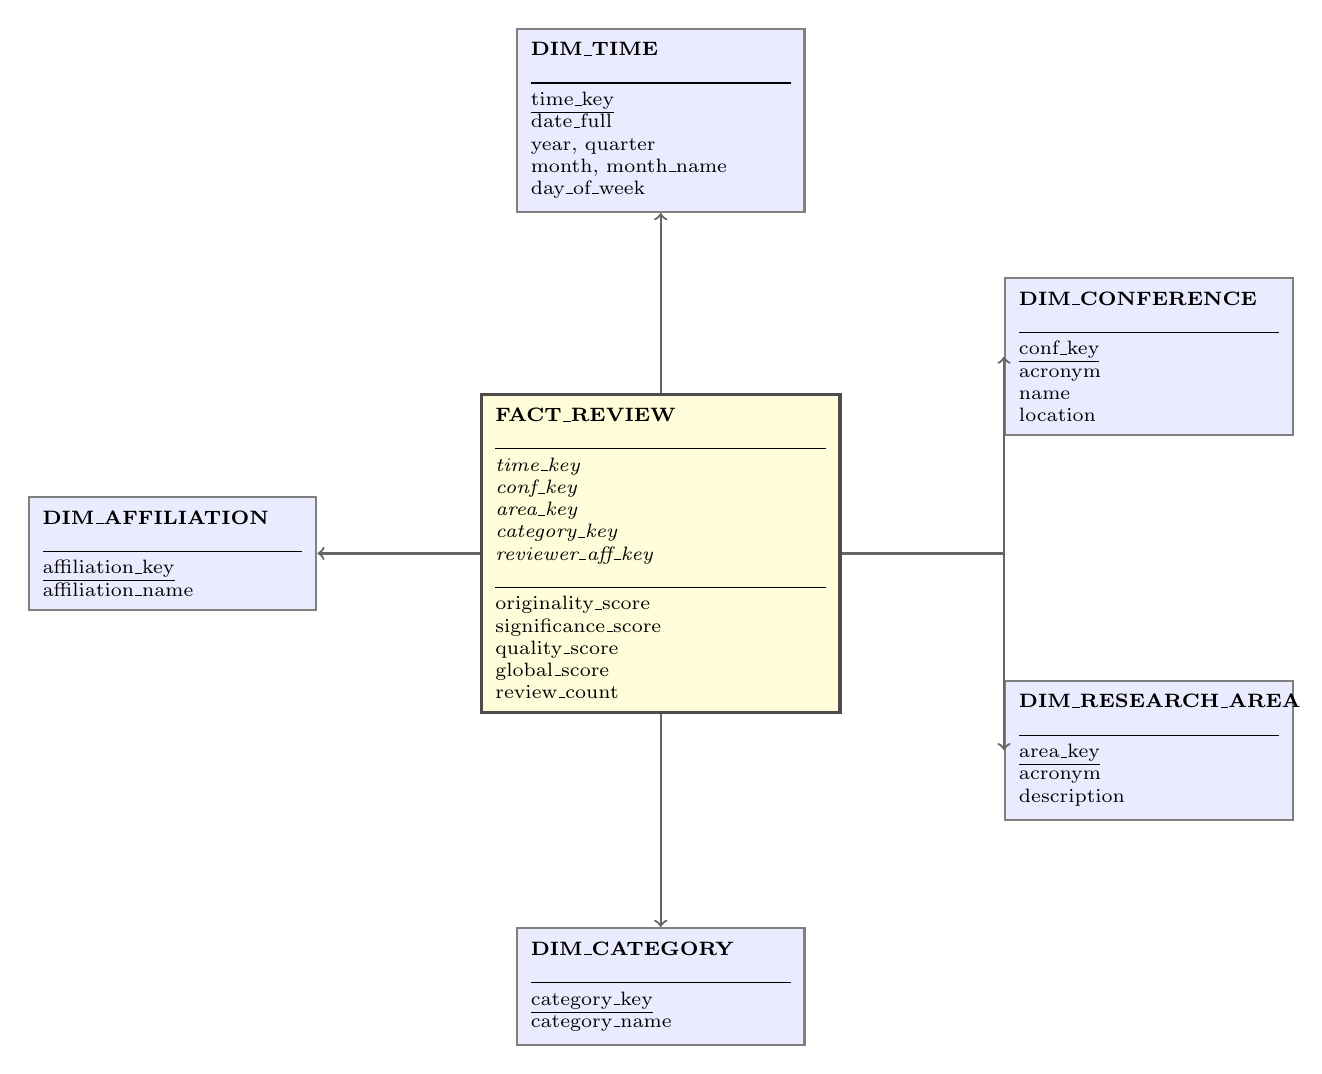
\begin{tikzpicture}[
    fact/.style={
        rectangle, draw=black!70, fill=yellow!15, very thick,
        text width=4.2cm, align=left, font=\scriptsize,
        inner sep=5pt
    },
    dim/.style={
        rectangle, draw=black!50, fill=blue!8, thick,
        text width=3.3cm, align=left, font=\scriptsize,
        inner sep=5pt
    },
    arr/.style={->, thick, black!60}
]

% --- Fact table (center) ---
\node[fact] (fact) at (0,0) {
    \textbf{FACT\_REVIEW} \\[2pt]
    \rule{\linewidth}{0.4pt} \\
    \textit{time\_key} \\
    \textit{conf\_key} \\
    \textit{area\_key} \\
    \textit{category\_key} \\
    \textit{reviewer\_aff\_key} \\[2pt]
    \rule{\linewidth}{0.4pt} \\
    originality\_score \\
    significance\_score \\
    quality\_score \\
    global\_score \\
    review\_count
};

% --- Dimensions ---
\node[dim] (time) at (0, 5.5) {
    \textbf{DIM\_TIME} \\[2pt]
    \rule{\linewidth}{0.4pt} \\
    \underline{time\_key} \\
    date\_full \\
    year, quarter \\
    month, month\_name \\
    day\_of\_week
};

\node[dim] (conf) at (6.2, 2.5) {
    \textbf{DIM\_CONFERENCE} \\[2pt]
    \rule{\linewidth}{0.4pt} \\
    \underline{conf\_key} \\
    acronym \\
    name \\
    location
};

\node[dim] (area) at (6.2, -2.5) {
    \textbf{DIM\_RESEARCH\_AREA} \\[2pt]
    \rule{\linewidth}{0.4pt} \\
    \underline{area\_key} \\
    acronym \\
    description
};

\node[dim] (cat) at (0, -5.5) {
    \textbf{DIM\_CATEGORY} \\[2pt]
    \rule{\linewidth}{0.4pt} \\
    \underline{category\_key} \\
    category\_name
};

\node[dim] (aff) at (-6.2, 0) {
    \textbf{DIM\_AFFILIATION} \\[2pt]
    \rule{\linewidth}{0.4pt} \\
    \underline{affiliation\_key} \\
    affiliation\_name
};

% --- Arrows (Fact -> Dim) ---
\draw[arr] (fact.north)  -- (time.south);
\draw[arr] (fact.east)   -| (conf.west);
\draw[arr] (fact.east)   -| (area.west);
\draw[arr] (fact.south)  -- (cat.north);
\draw[arr] (fact.west)   -- (aff.east);

\end{tikzpicture}
\caption{Star Schema for FACT\_REVIEW.}
\label{fig:star_schema}
\end{figure}

\begin{figure}[!ht]
\centering
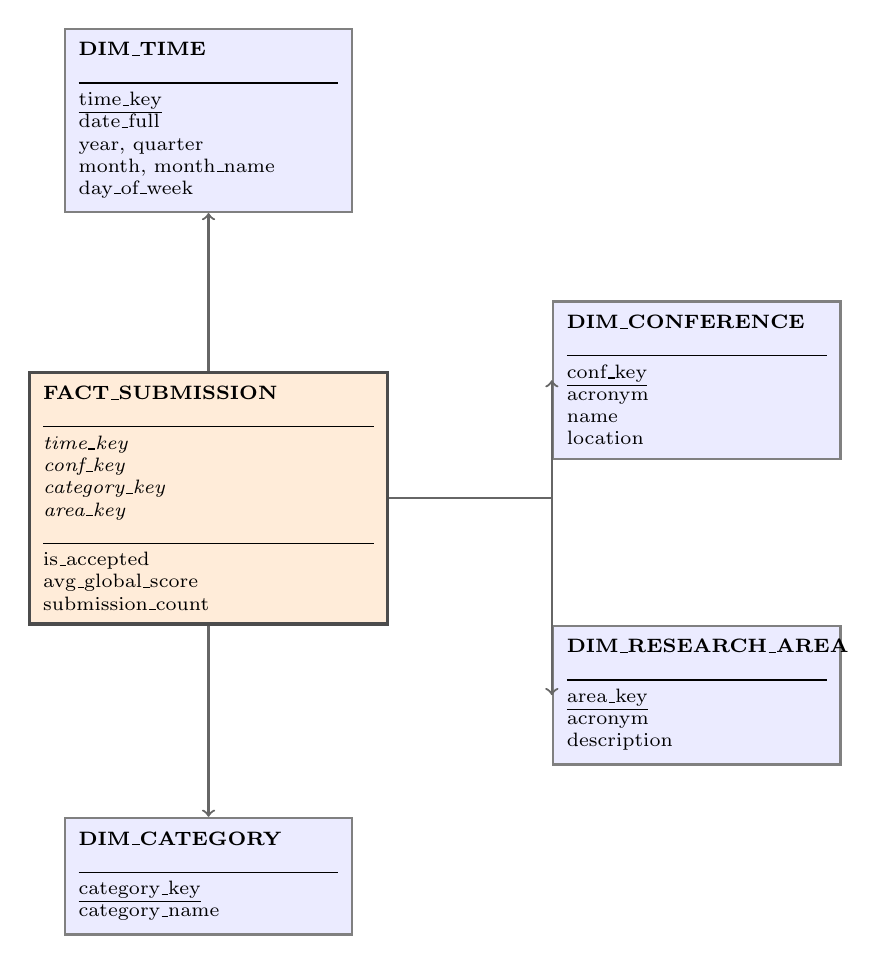
\begin{tikzpicture}[
    fact/.style={
        rectangle, draw=black!70, fill=orange!15, very thick,
        text width=4.2cm, align=left, font=\scriptsize,
        inner sep=5pt
    },
    dim/.style={
        rectangle, draw=black!50, fill=blue!8, thick,
        text width=3.3cm, align=left, font=\scriptsize,
        inner sep=5pt
    },
    arr/.style={->, thick, black!60}
]

% --- Fact table (center) ---
\node[fact] (fact2) at (0,0) {
    \textbf{FACT\_SUBMISSION} \\[2pt]
    \rule{\linewidth}{0.4pt} \\
    \textit{time\_key} \\
    \textit{conf\_key} \\
    \textit{category\_key} \\
    \textit{area\_key} \\[2pt]
    \rule{\linewidth}{0.4pt} \\
    is\_accepted \\
    avg\_global\_score \\
    submission\_count
};

% --- Dimensions ---
\node[dim] (time2) at (0, 4.8) {
    \textbf{DIM\_TIME} \\[2pt]
    \rule{\linewidth}{0.4pt} \\
    \underline{time\_key} \\
    date\_full \\
    year, quarter \\
    month, month\_name \\
    day\_of\_week
};

\node[dim] (conf2) at (6.2, 1.5) {
    \textbf{DIM\_CONFERENCE} \\[2pt]
    \rule{\linewidth}{0.4pt} \\
    \underline{conf\_key} \\
    acronym \\
    name \\
    location
};

\node[dim] (area2) at (6.2, -2.5) {
    \textbf{DIM\_RESEARCH\_AREA} \\[2pt]
    \rule{\linewidth}{0.4pt} \\
    \underline{area\_key} \\
    acronym \\
    description
};

\node[dim] (cat2) at (0, -4.8) {
    \textbf{DIM\_CATEGORY} \\[2pt]
    \rule{\linewidth}{0.4pt} \\
    \underline{category\_key} \\
    category\_name
};

% --- Arrows (Fact -> Dim) ---
\draw[arr] (fact2.north)  -- (time2.south);
\draw[arr] (fact2.east)   -| (conf2.west);
\draw[arr] (fact2.east)   -| (area2.west);
\draw[arr] (fact2.south)  -- (cat2.north);

\end{tikzpicture}
\caption{Star Schema for FACT\_SUBMISSION.}
\label{fig:star_schema_submission}
\end{figure}

\begin{infobox}
FACT\_SUBMISSION does not have a link to DIM\_AFFILIATION because submissions are not tied to a specific reviewer. The two fact tables share the other four dimensions, forming a \emph{constellation schema} (also called galaxy schema).
\end{infobox}

\section{ETL Process}

Data is moved from the operational database to the DW through an ETL (Extract, Transform, Load) process:

\begin{enumerate}
  \item \textbf{Extract}: read new or updated rows from the OLTP tables (Conference, Article, Review, Organizer).
  \item \textbf{Transform}: map natural keys to surrogate keys, compute derived fields like \texttt{is\_accepted}, and extract time components from dates.
  \item \textbf{Load}: insert the transformed rows into the fact and dimension tables.
\end{enumerate}

\begin{infobox}
The ETL runs as a nightly batch job. Real-time updates are not needed because analytical queries are typically run on a daily or weekly basis.
\end{infobox}

\section{OLAP Operations}

With the star schema in place, analysts can perform standard OLAP operations:

\begin{table}[!ht]
\centering
\caption{Standard OLAP operations.}
\label{tab:olap_ops}
\small
\begin{tabularx}{\textwidth}{@{} l X l @{}}
  \toprule
  Operation & What it does & Example \\
  \midrule
  Roll-up    & Go from detail to summary.              & Monthly $\rightarrow$ yearly avg score \\
  Drill-down & Go from summary to detail.              & Conference $\rightarrow$ category level \\
  Slice      & Filter on one dimension.                & Only year 2025 \\
  Dice       & Filter on multiple dimensions.          & Year 2025, location ``Bari'' \\
  Pivot      & Swap rows and columns.                  & Rows = area, Columns = year \\
  \bottomrule
\end{tabularx}
\end{table}


% --- Conclusions ---
% \include{chapters/conclusions}

% --- Bibliography ---
% \bibliographystyle{plain}
% \bibliography{references}

\end{document}
